\documentclass[a4paper]{book}
\usepackage{makeidx}
\usepackage{natbib}
\usepackage{graphicx}
\usepackage{multicol}
\usepackage{float}
\usepackage{listings}
\usepackage{color}
\usepackage{ifthen}
\usepackage[table]{xcolor}
\usepackage{textcomp}
\usepackage{alltt}
\usepackage{ifpdf}
\ifpdf
\usepackage[pdftex,
            pagebackref=true,
            colorlinks=true,
            linkcolor=blue,
            unicode
           ]{hyperref}
\else
\usepackage[ps2pdf,
            pagebackref=true,
            colorlinks=true,
            linkcolor=blue,
            unicode
           ]{hyperref}
\usepackage{pspicture}
\fi
\usepackage[utf8]{inputenc}
\usepackage{mathptmx}
\usepackage[scaled=.90]{helvet}
\usepackage{courier}
\usepackage{sectsty}
\usepackage[titles]{tocloft}
\usepackage{doxygen}
\lstset{language=C++,inputencoding=utf8,basicstyle=\footnotesize,breaklines=true,breakatwhitespace=true,tabsize=8,numbers=left }
\makeindex
\setcounter{tocdepth}{3}
\renewcommand{\footrulewidth}{0.4pt}
\renewcommand{\familydefault}{\sfdefault}
\hfuzz=15pt
\setlength{\emergencystretch}{15pt}
\hbadness=750
\tolerance=750
\begin{document}
\hypersetup{pageanchor=false,citecolor=blue}
\begin{titlepage}
\vspace*{7cm}
\begin{center}
{\Large \-Spec -\/ specialitky ve \-Fortranu }\\
\vspace*{1cm}
{\large \-Generated by Doxygen 1.7.6.1}\\
\vspace*{0.5cm}
{\small Sun Sep 1 2013 11:32:27}\\
\end{center}
\end{titlepage}
\clearemptydoublepage
\pagenumbering{roman}
\tableofcontents
\clearemptydoublepage
\pagenumbering{arabic}
\hypersetup{pageanchor=true,citecolor=blue}
\chapter{\-Data \-Type \-Index}
\section{\-Class \-Hierarchy}
\-This inheritance list is sorted roughly, but not completely, alphabetically\-:\begin{DoxyCompactList}
\item \contentsline{section}{datasetup}{\pageref{classdatasetup}}{}
\item \contentsline{section}{mtx\-:\-:elemt}{\pageref{structmtx_1_1elemt}}{}
\item \contentsline{section}{mtx\-:\-:geti}{\pageref{interfacemtx_1_1geti}}{}
\item \contentsline{section}{mtx\-:\-:ini}{\pageref{interfacemtx_1_1ini}}{}
\item \contentsline{section}{mtx\-:\-:matrix}{\pageref{structmtx_1_1matrix}}{}
\begin{DoxyCompactList}
\item \contentsline{section}{mtx\-:\-:fullmtx}{\pageref{structmtx_1_1fullmtx}}{}
\item \contentsline{section}{mtx\-:\-:smtx}{\pageref{structmtx_1_1smtx}}{}
\end{DoxyCompactList}
\item \contentsline{section}{mtx}{\pageref{classmtx}}{}
\item \contentsline{section}{mtx\-:\-:seti}{\pageref{interfacemtx_1_1seti}}{}
\item \contentsline{section}{solvers}{\pageref{classsolvers}}{}
\item \contentsline{section}{typy\-:\-:tcount}{\pageref{structtypy_1_1tcount}}{}
\item \contentsline{section}{typy}{\pageref{classtypy}}{}
\end{DoxyCompactList}

\chapter{\-Data \-Type \-Index}
\section{\-Data \-Types \-List}
\-Here are the data types with brief descriptions\-:\begin{DoxyCompactList}
\item\contentsline{section}{\hyperlink{classdatasetup}{datasetup} \\*\-Konstruktory matic }{\pageref{classdatasetup}}{}
\item\contentsline{section}{\hyperlink{structmtx_1_1elemt}{mtx\-::elemt} \\*\-Typ pro prvek ridke matice }{\pageref{structmtx_1_1elemt}}{}
\item\contentsline{section}{\hyperlink{structmtx_1_1fullmtx}{mtx\-::fullmtx} \\*\-Plna matice }{\pageref{structmtx_1_1fullmtx}}{}
\item\contentsline{section}{\hyperlink{interfacemtx_1_1geti}{mtx\-::geti} \\*\-Interface pro ziskani prvku }{\pageref{interfacemtx_1_1geti}}{}
\item\contentsline{section}{\hyperlink{interfacemtx_1_1ini}{mtx\-::ini} \\*\-Interface pro inicializaci=vymazani matice a resize }{\pageref{interfacemtx_1_1ini}}{}
\item\contentsline{section}{\hyperlink{structmtx_1_1matrix}{mtx\-::matrix} \\*\-Obecna matice }{\pageref{structmtx_1_1matrix}}{}
\item\contentsline{section}{\hyperlink{classmtx}{mtx} \\*\-Module pro matice }{\pageref{classmtx}}{}
\item\contentsline{section}{\hyperlink{interfacemtx_1_1seti}{mtx\-::seti} \\*\-Interface pro nastaveni prvku }{\pageref{interfacemtx_1_1seti}}{}
\item\contentsline{section}{\hyperlink{structmtx_1_1smtx}{mtx\-::smtx} \\*\-Ridka matice }{\pageref{structmtx_1_1smtx}}{}
\item\contentsline{section}{\hyperlink{classsolvers}{solvers} \\*\-Resice soustav }{\pageref{classsolvers}}{}
\item\contentsline{section}{\hyperlink{structtypy_1_1tcount}{typy\-::tcount} \\*\-Pocitadlo operaci }{\pageref{structtypy_1_1tcount}}{}
\item\contentsline{section}{\hyperlink{classtypy}{typy} \\*\-Zakladni typy }{\pageref{classtypy}}{}
\end{DoxyCompactList}

\chapter{\-File \-Index}
\section{\-File \-List}
\-Here is a list of all files with brief descriptions\-:\begin{DoxyCompactList}
\item\contentsline{section}{\hyperlink{datasetup_8f90}{datasetup.\-f90} \\*\-Konstruktory matic }{\pageref{datasetup_8f90}}{}
\item\contentsline{section}{\hyperlink{main_8f90}{main.\-f90} \\*\-Hlavni program }{\pageref{main_8f90}}{}
\item\contentsline{section}{\hyperlink{mtx_8f90}{mtx.\-f90} \\*\-Objektova implementace matic }{\pageref{mtx_8f90}}{}
\item\contentsline{section}{\hyperlink{solvers_8f90}{solvers.\-f90} \\*\-Ruzne resice soustav linearnich rovnic }{\pageref{solvers_8f90}}{}
\item\contentsline{section}{\hyperlink{typy_8f90}{typy.\-f90} \\*\-Modul pro zakladni typy }{\pageref{typy_8f90}}{}
\end{DoxyCompactList}

\chapter{\-Data \-Type \-Documentation}
\hypertarget{classdatasetup}{\section{datasetup \-Module \-Reference}
\label{classdatasetup}\index{datasetup@{datasetup}}
}


konstruktory matic  


\subsection*{\-Public \-Member \-Functions}
\begin{DoxyCompactItemize}
\item 
subroutine, public \hyperlink{classdatasetup_a2426944a14260f1d4a9651071a0151ce}{\-Laplace2\-D} (a, nx, ny)
\begin{DoxyCompactList}\small\item\em diskretizace 2\-D \-Laplaceova operatoru \end{DoxyCompactList}\end{DoxyCompactItemize}


\subsection{\-Detailed \-Description}
konstruktory matic 

\-Definition at line 6 of file datasetup.\-f90.



\subsection{\-Member \-Function/\-Subroutine \-Documentation}
\hypertarget{classdatasetup_a2426944a14260f1d4a9651071a0151ce}{\index{datasetup@{datasetup}!\-Laplace2\-D@{\-Laplace2\-D}}
\index{\-Laplace2\-D@{\-Laplace2\-D}!datasetup@{datasetup}}
\subsubsection[{\-Laplace2\-D}]{\setlength{\rightskip}{0pt plus 5cm}subroutine, public {\bf datasetup\-::\-Laplace2\-D} (
\begin{DoxyParamCaption}
\item[{class(matrix), intent(inout)}]{a, }
\item[{integer(kind=ikind), intent(in)}]{nx, }
\item[{integer(kind=ikind), intent(in)}]{ny}
\end{DoxyParamCaption}
)}}\label{classdatasetup_a2426944a14260f1d4a9651071a0151ce}


diskretizace 2\-D \-Laplaceova operatoru 

sit je rovnomerna s krokem h=1/nxpr 
\begin{DoxyParams}[1]{\-Parameters}
\mbox{\tt in,out}  & {\em a} & vytvarena matice \\
\hline
\mbox{\tt in}  & {\em nx} & pocet uzlu ve smeru x \\
\hline
\mbox{\tt in}  & {\em ny} & pocet uzlu ve smeru y \\
\hline
\end{DoxyParams}


\-Definition at line 14 of file datasetup.\-f90.



\-The documentation for this module was generated from the following file\-:\begin{DoxyCompactItemize}
\item 
\hyperlink{datasetup_8f90}{datasetup.\-f90}\end{DoxyCompactItemize}

\hypertarget{structmtx_1_1elemt}{\section{mtx\-:\-:elemt \-Type \-Reference}
\label{structmtx_1_1elemt}\index{mtx\-::elemt@{mtx\-::elemt}}
}


typ pro prvek ridke matice  




\-Collaboration diagram for mtx\-:\-:elemt\-:\nopagebreak
\begin{figure}[H]
\begin{center}
\leavevmode
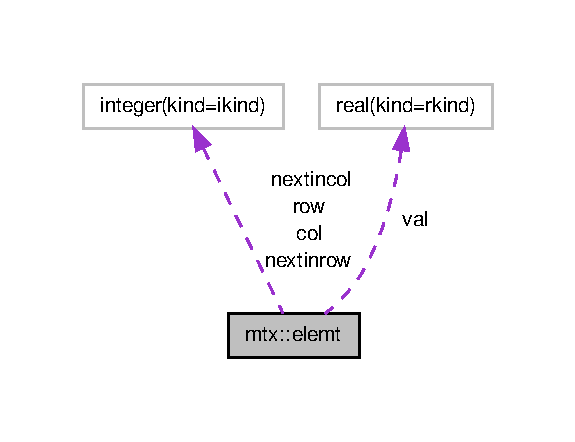
\includegraphics[width=276pt]{structmtx_1_1elemt__coll__graph}
\end{center}
\end{figure}
\subsection*{\-Public \-Attributes}
\begin{DoxyCompactItemize}
\item 
real(kind=rkind) \hyperlink{structmtx_1_1elemt_ad16a0504f754e953a16926f9414e12b5}{val} = 0
\begin{DoxyCompactList}\small\item\em hodnota \end{DoxyCompactList}\item 
integer(kind=ikind) \hyperlink{structmtx_1_1elemt_aa2b8f13c3e5c242af5d3d6a13f0deecf}{row} = 0
\begin{DoxyCompactList}\small\item\em radek \end{DoxyCompactList}\item 
integer(kind=ikind) \hyperlink{structmtx_1_1elemt_ae051633c302f8ceebc82d612c74ac62f}{col} = 0
\begin{DoxyCompactList}\small\item\em sloupec \end{DoxyCompactList}\item 
integer(kind=ikind) \hyperlink{structmtx_1_1elemt_a49dfbfe79b719bc8c5d7678809b799b7}{nextinrow} = -\/1
\begin{DoxyCompactList}\small\item\em index dalsiho prvku v radku pokud zadny neni = -\/1 \end{DoxyCompactList}\item 
integer(kind=ikind) \hyperlink{structmtx_1_1elemt_a2a4b03e64a45c4349c06a426a0e3e064}{nextincol} = -\/1
\begin{DoxyCompactList}\small\item\em index dalsiho prvku ve sloupci pokud zadny neni = -\/1 \end{DoxyCompactList}\end{DoxyCompactItemize}


\subsection{\-Detailed \-Description}
typ pro prvek ridke matice 

\-Definition at line 105 of file mtx.\-f90.



\subsection{\-Member \-Data \-Documentation}
\hypertarget{structmtx_1_1elemt_ae051633c302f8ceebc82d612c74ac62f}{\index{mtx\-::elemt@{mtx\-::elemt}!col@{col}}
\index{col@{col}!mtx::elemt@{mtx\-::elemt}}
\subsubsection[{col}]{\setlength{\rightskip}{0pt plus 5cm}integer(kind=ikind) {\bf mtx\-::elemt\-::col} = 0}}\label{structmtx_1_1elemt_ae051633c302f8ceebc82d612c74ac62f}


sloupec 



\-Definition at line 111 of file mtx.\-f90.

\hypertarget{structmtx_1_1elemt_a2a4b03e64a45c4349c06a426a0e3e064}{\index{mtx\-::elemt@{mtx\-::elemt}!nextincol@{nextincol}}
\index{nextincol@{nextincol}!mtx::elemt@{mtx\-::elemt}}
\subsubsection[{nextincol}]{\setlength{\rightskip}{0pt plus 5cm}integer(kind=ikind) {\bf mtx\-::elemt\-::nextincol} = -\/1}}\label{structmtx_1_1elemt_a2a4b03e64a45c4349c06a426a0e3e064}


index dalsiho prvku ve sloupci pokud zadny neni = -\/1 



\-Definition at line 115 of file mtx.\-f90.

\hypertarget{structmtx_1_1elemt_a49dfbfe79b719bc8c5d7678809b799b7}{\index{mtx\-::elemt@{mtx\-::elemt}!nextinrow@{nextinrow}}
\index{nextinrow@{nextinrow}!mtx::elemt@{mtx\-::elemt}}
\subsubsection[{nextinrow}]{\setlength{\rightskip}{0pt plus 5cm}integer(kind=ikind) {\bf mtx\-::elemt\-::nextinrow} = -\/1}}\label{structmtx_1_1elemt_a49dfbfe79b719bc8c5d7678809b799b7}


index dalsiho prvku v radku pokud zadny neni = -\/1 



\-Definition at line 113 of file mtx.\-f90.

\hypertarget{structmtx_1_1elemt_aa2b8f13c3e5c242af5d3d6a13f0deecf}{\index{mtx\-::elemt@{mtx\-::elemt}!row@{row}}
\index{row@{row}!mtx::elemt@{mtx\-::elemt}}
\subsubsection[{row}]{\setlength{\rightskip}{0pt plus 5cm}integer(kind=ikind) {\bf mtx\-::elemt\-::row} = 0}}\label{structmtx_1_1elemt_aa2b8f13c3e5c242af5d3d6a13f0deecf}


radek 



\-Definition at line 109 of file mtx.\-f90.

\hypertarget{structmtx_1_1elemt_ad16a0504f754e953a16926f9414e12b5}{\index{mtx\-::elemt@{mtx\-::elemt}!val@{val}}
\index{val@{val}!mtx::elemt@{mtx\-::elemt}}
\subsubsection[{val}]{\setlength{\rightskip}{0pt plus 5cm}real(kind=rkind) {\bf mtx\-::elemt\-::val} = 0}}\label{structmtx_1_1elemt_ad16a0504f754e953a16926f9414e12b5}


hodnota 



\-Definition at line 107 of file mtx.\-f90.



\-The documentation for this type was generated from the following file\-:\begin{DoxyCompactItemize}
\item 
\hyperlink{mtx_8f90}{mtx.\-f90}\end{DoxyCompactItemize}

\hypertarget{structmtx_1_1fullmtx}{\section{mtx\-:\-:fullmtx \-Type \-Reference}
\label{structmtx_1_1fullmtx}\index{mtx\-::fullmtx@{mtx\-::fullmtx}}
}


plna matice  




\-Inheritance diagram for mtx\-:\-:fullmtx\-:\nopagebreak
\begin{figure}[H]
\begin{center}
\leavevmode
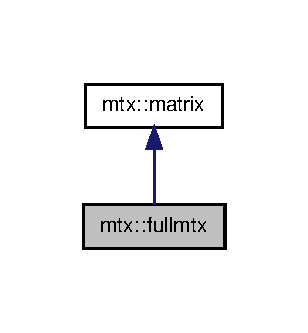
\includegraphics[width=148pt]{structmtx_1_1fullmtx__inherit__graph}
\end{center}
\end{figure}


\-Collaboration diagram for mtx\-:\-:fullmtx\-:
\nopagebreak
\begin{figure}[H]
\begin{center}
\leavevmode
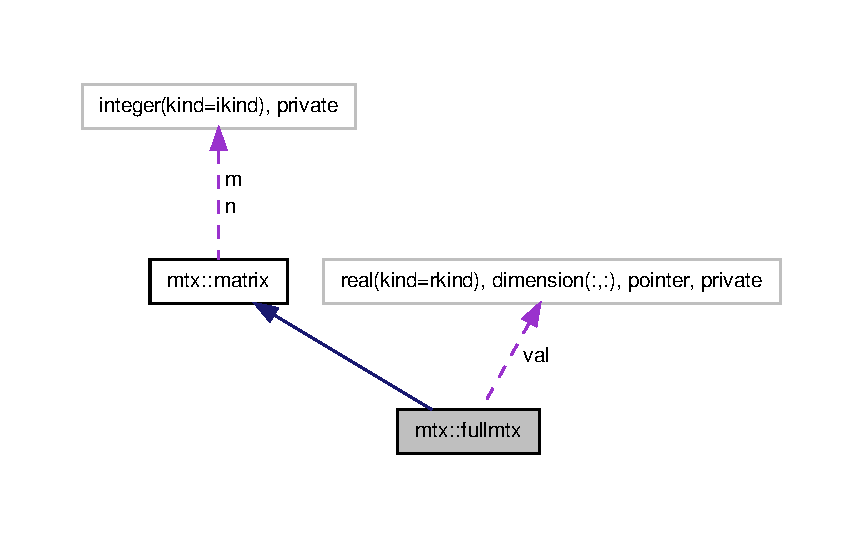
\includegraphics[width=350pt]{structmtx_1_1fullmtx__coll__graph}
\end{center}
\end{figure}
\subsection*{\-Public \-Member \-Functions}
\begin{DoxyCompactItemize}
\item 
procedure \hyperlink{structmtx_1_1fullmtx_a61b753f6a76bcfd96fbe82c26bbdce8b}{init} =$>$ \hyperlink{classmtx_a9d997a2261d0627633b50e21779cafeb}{initfull}
\begin{DoxyCompactList}\small\item\em inicializace matice \end{DoxyCompactList}\item 
procedure \hyperlink{structmtx_1_1fullmtx_a2155f93b9fceea289c90e7f01fb505a7}{get} =$>$ \hyperlink{classmtx_a19fea5b5c69870346797740e80888c31}{getfull}
\begin{DoxyCompactList}\small\item\em vrati prvek matice \end{DoxyCompactList}\item 
procedure, pass(a) \hyperlink{structmtx_1_1fullmtx_ac28edc8d06a554863016c1e369d218c4}{set} =$>$ \hyperlink{classmtx_ad535bdf867ccb7c8e9b27f17609e6517}{setfull}
\begin{DoxyCompactList}\small\item\em nastavi prvek matice \end{DoxyCompactList}\item 
procedure, non\-\_\-overridable \hyperlink{structmtx_1_1matrix_ad43a73f32b347da18f997ce145d6c27c}{getn} =$>$ \hyperlink{classmtx_ab05f486a31448c69570e2144b4010957}{getnmatrix}
\begin{DoxyCompactList}\small\item\em vrati pocet radku \end{DoxyCompactList}\item 
procedure, non\-\_\-overridable \hyperlink{structmtx_1_1matrix_a24f1071ad0cb83094ba23d3027321392}{getm} =$>$ \hyperlink{classmtx_adf266f7c4ef90f6ddc1c654bcad5d149}{getmmatrix}
\begin{DoxyCompactList}\small\item\em vrati pocet sloupcu \end{DoxyCompactList}\item 
procedure \hyperlink{structmtx_1_1matrix_a99c4dff8cf1c63a968d03474084d0b70}{getrow} =$>$ \hyperlink{classmtx_a46e5fd9002257990ea5c79e1971c8167}{getrowmatrix}
\begin{DoxyCompactList}\small\item\em vybere radek z matice \end{DoxyCompactList}\item 
procedure \hyperlink{structmtx_1_1matrix_af9d60c003f797c73085241d8c38ea792}{getcol} =$>$ \hyperlink{classmtx_abb68e8d5a8216a50b88e5c577b5ad403}{getcolmatrix}
\begin{DoxyCompactList}\small\item\em vybere sloupec z matice \end{DoxyCompactList}\item 
procedure \hyperlink{structmtx_1_1matrix_a4b7b05cc668bbeffed54335122063a03}{print} =$>$ \hyperlink{classmtx_a9b242fed3892da977edee5be16d85bdf}{printmatrix}
\begin{DoxyCompactList}\small\item\em vytiskne matici \end{DoxyCompactList}\item 
procedure \hyperlink{structmtx_1_1matrix_a1eacf25c7fa77ff8766a1ab281f50f19}{dump} =$>$ \hyperlink{classmtx_ae8163b304193b3e31cc36e31113ec9e9}{dumpmatrix}
\begin{DoxyCompactList}\small\item\em dumpne celou strukturu matice \end{DoxyCompactList}\item 
procedure \hyperlink{structmtx_1_1matrix_a085ae99f3dbc3a44fc4eba9471827fd9}{nonzero} =$>$ \hyperlink{classmtx_aac2e9af9cc01d6d2e4c305eb6ba95b7c}{nzmatrix}
\begin{DoxyCompactList}\small\item\em da pocet nenul v matici \end{DoxyCompactList}\item 
procedure, non\-\_\-overridable \hyperlink{structmtx_1_1matrix_a244598586f2b4d2de61eb827c6349485}{spy} =$>$ \hyperlink{classmtx_afba151bbf31e292a36f36279c0d74cf2}{spymatrix}
\begin{DoxyCompactList}\small\item\em textova varianta spy \end{DoxyCompactList}\item 
procedure \hyperlink{structmtx_1_1matrix_acb57be54454a5c1fad3429d8fab32b95}{mul} =$>$ \hyperlink{classmtx_a33216e985c0e2ec6536c2f013f8562ac}{mulmatrix}
\begin{DoxyCompactList}\small\item\em nasobi vektorem \end{DoxyCompactList}\item 
procedure \hyperlink{structmtx_1_1matrix_a54be9493d99d3be7246d31d46e21fd72}{copy} =$>$ \hyperlink{classmtx_add2b7c4a3a806aebca088907544db1e0}{copymatrix}
\begin{DoxyCompactList}\small\item\em udela kopii matice \end{DoxyCompactList}\end{DoxyCompactItemize}
\subsection*{\-Private \-Attributes}
\begin{DoxyCompactItemize}
\item 
real(kind=rkind), dimension(\-:,\-:), \*
pointer, private \hyperlink{structmtx_1_1fullmtx_a5afa79f4180ded442b60ee854b636b36}{val} = $>$ null()
\begin{DoxyCompactList}\small\item\em hodnoty prvku \end{DoxyCompactList}\end{DoxyCompactItemize}


\subsection{\-Detailed \-Description}
plna matice 

\-Definition at line 95 of file mtx.\-f90.



\subsection{\-Member \-Function/\-Subroutine \-Documentation}
\hypertarget{structmtx_1_1matrix_a54be9493d99d3be7246d31d46e21fd72}{\index{mtx\-::fullmtx@{mtx\-::fullmtx}!copy@{copy}}
\index{copy@{copy}!mtx::fullmtx@{mtx\-::fullmtx}}
\subsubsection[{copy}]{\setlength{\rightskip}{0pt plus 5cm}procedure {\bf mtx\-::matrix\-::copy} (
\begin{DoxyParamCaption}
{}
\end{DoxyParamCaption}
)\hspace{0.3cm}{\ttfamily  \mbox{[}inherited\mbox{]}}}}\label{structmtx_1_1matrix_a54be9493d99d3be7246d31d46e21fd72}


udela kopii matice 



\-Definition at line 44 of file mtx.\-f90.

\hypertarget{structmtx_1_1matrix_a1eacf25c7fa77ff8766a1ab281f50f19}{\index{mtx\-::fullmtx@{mtx\-::fullmtx}!dump@{dump}}
\index{dump@{dump}!mtx::fullmtx@{mtx\-::fullmtx}}
\subsubsection[{dump}]{\setlength{\rightskip}{0pt plus 5cm}procedure {\bf mtx\-::matrix\-::dump} (
\begin{DoxyParamCaption}
{}
\end{DoxyParamCaption}
)\hspace{0.3cm}{\ttfamily  \mbox{[}inherited\mbox{]}}}}\label{structmtx_1_1matrix_a1eacf25c7fa77ff8766a1ab281f50f19}


dumpne celou strukturu matice 



\-Reimplemented in \hyperlink{structmtx_1_1smtx_ac7863d852b3115cf545f7ed8356be3fc}{mtx\-::smtx}.



\-Definition at line 36 of file mtx.\-f90.

\hypertarget{structmtx_1_1fullmtx_a2155f93b9fceea289c90e7f01fb505a7}{\index{mtx\-::fullmtx@{mtx\-::fullmtx}!get@{get}}
\index{get@{get}!mtx::fullmtx@{mtx\-::fullmtx}}
\subsubsection[{get}]{\setlength{\rightskip}{0pt plus 5cm}procedure {\bf mtx\-::fullmtx\-::get} (
\begin{DoxyParamCaption}
{}
\end{DoxyParamCaption}
)}}\label{structmtx_1_1fullmtx_a2155f93b9fceea289c90e7f01fb505a7}


vrati prvek matice 



\-Reimplemented from \hyperlink{structmtx_1_1matrix_aefbbd3d12a8d6429c183bec463749bda}{mtx\-::matrix}.



\-Definition at line 100 of file mtx.\-f90.

\hypertarget{structmtx_1_1matrix_af9d60c003f797c73085241d8c38ea792}{\index{mtx\-::fullmtx@{mtx\-::fullmtx}!getcol@{getcol}}
\index{getcol@{getcol}!mtx::fullmtx@{mtx\-::fullmtx}}
\subsubsection[{getcol}]{\setlength{\rightskip}{0pt plus 5cm}procedure {\bf mtx\-::matrix\-::getcol} (
\begin{DoxyParamCaption}
{}
\end{DoxyParamCaption}
)\hspace{0.3cm}{\ttfamily  \mbox{[}inherited\mbox{]}}}}\label{structmtx_1_1matrix_af9d60c003f797c73085241d8c38ea792}


vybere sloupec z matice 



\-Definition at line 32 of file mtx.\-f90.

\hypertarget{structmtx_1_1matrix_a24f1071ad0cb83094ba23d3027321392}{\index{mtx\-::fullmtx@{mtx\-::fullmtx}!getm@{getm}}
\index{getm@{getm}!mtx::fullmtx@{mtx\-::fullmtx}}
\subsubsection[{getm}]{\setlength{\rightskip}{0pt plus 5cm}procedure, non\-\_\-overridable {\bf mtx\-::matrix\-::getm} (
\begin{DoxyParamCaption}
{}
\end{DoxyParamCaption}
)\hspace{0.3cm}{\ttfamily  \mbox{[}inherited\mbox{]}}}}\label{structmtx_1_1matrix_a24f1071ad0cb83094ba23d3027321392}


vrati pocet sloupcu 



\-Definition at line 22 of file mtx.\-f90.

\hypertarget{structmtx_1_1matrix_ad43a73f32b347da18f997ce145d6c27c}{\index{mtx\-::fullmtx@{mtx\-::fullmtx}!getn@{getn}}
\index{getn@{getn}!mtx::fullmtx@{mtx\-::fullmtx}}
\subsubsection[{getn}]{\setlength{\rightskip}{0pt plus 5cm}procedure, non\-\_\-overridable {\bf mtx\-::matrix\-::getn} (
\begin{DoxyParamCaption}
{}
\end{DoxyParamCaption}
)\hspace{0.3cm}{\ttfamily  \mbox{[}inherited\mbox{]}}}}\label{structmtx_1_1matrix_ad43a73f32b347da18f997ce145d6c27c}


vrati pocet radku 



\-Definition at line 20 of file mtx.\-f90.

\hypertarget{structmtx_1_1matrix_a99c4dff8cf1c63a968d03474084d0b70}{\index{mtx\-::fullmtx@{mtx\-::fullmtx}!getrow@{getrow}}
\index{getrow@{getrow}!mtx::fullmtx@{mtx\-::fullmtx}}
\subsubsection[{getrow}]{\setlength{\rightskip}{0pt plus 5cm}procedure {\bf mtx\-::matrix\-::getrow} (
\begin{DoxyParamCaption}
{}
\end{DoxyParamCaption}
)\hspace{0.3cm}{\ttfamily  \mbox{[}inherited\mbox{]}}}}\label{structmtx_1_1matrix_a99c4dff8cf1c63a968d03474084d0b70}


vybere radek z matice 



\-Definition at line 30 of file mtx.\-f90.

\hypertarget{structmtx_1_1fullmtx_a61b753f6a76bcfd96fbe82c26bbdce8b}{\index{mtx\-::fullmtx@{mtx\-::fullmtx}!init@{init}}
\index{init@{init}!mtx::fullmtx@{mtx\-::fullmtx}}
\subsubsection[{init}]{\setlength{\rightskip}{0pt plus 5cm}procedure {\bf mtx\-::fullmtx\-::init} (
\begin{DoxyParamCaption}
{}
\end{DoxyParamCaption}
)}}\label{structmtx_1_1fullmtx_a61b753f6a76bcfd96fbe82c26bbdce8b}


inicializace matice 



\-Reimplemented from \hyperlink{structmtx_1_1matrix_a93ca8f74b8962073bdde2cf422abd191}{mtx\-::matrix}.



\-Definition at line 99 of file mtx.\-f90.

\hypertarget{structmtx_1_1matrix_acb57be54454a5c1fad3429d8fab32b95}{\index{mtx\-::fullmtx@{mtx\-::fullmtx}!mul@{mul}}
\index{mul@{mul}!mtx::fullmtx@{mtx\-::fullmtx}}
\subsubsection[{mul}]{\setlength{\rightskip}{0pt plus 5cm}procedure {\bf mtx\-::matrix\-::mul} (
\begin{DoxyParamCaption}
{}
\end{DoxyParamCaption}
)\hspace{0.3cm}{\ttfamily  \mbox{[}inherited\mbox{]}}}}\label{structmtx_1_1matrix_acb57be54454a5c1fad3429d8fab32b95}


nasobi vektorem 



\-Reimplemented in \hyperlink{structmtx_1_1smtx_a799fca1825561095bdb5a3342fb88a21}{mtx\-::smtx}.



\-Definition at line 42 of file mtx.\-f90.

\hypertarget{structmtx_1_1matrix_a085ae99f3dbc3a44fc4eba9471827fd9}{\index{mtx\-::fullmtx@{mtx\-::fullmtx}!nonzero@{nonzero}}
\index{nonzero@{nonzero}!mtx::fullmtx@{mtx\-::fullmtx}}
\subsubsection[{nonzero}]{\setlength{\rightskip}{0pt plus 5cm}procedure {\bf mtx\-::matrix\-::nonzero} (
\begin{DoxyParamCaption}
{}
\end{DoxyParamCaption}
)\hspace{0.3cm}{\ttfamily  \mbox{[}inherited\mbox{]}}}}\label{structmtx_1_1matrix_a085ae99f3dbc3a44fc4eba9471827fd9}


da pocet nenul v matici 



\-Reimplemented in \hyperlink{structmtx_1_1smtx_a6f111e4bbdebc5c728e9064be2164b65}{mtx\-::smtx}.



\-Definition at line 38 of file mtx.\-f90.

\hypertarget{structmtx_1_1matrix_a4b7b05cc668bbeffed54335122063a03}{\index{mtx\-::fullmtx@{mtx\-::fullmtx}!print@{print}}
\index{print@{print}!mtx::fullmtx@{mtx\-::fullmtx}}
\subsubsection[{print}]{\setlength{\rightskip}{0pt plus 5cm}procedure {\bf mtx\-::matrix\-::print} (
\begin{DoxyParamCaption}
{}
\end{DoxyParamCaption}
)\hspace{0.3cm}{\ttfamily  \mbox{[}inherited\mbox{]}}}}\label{structmtx_1_1matrix_a4b7b05cc668bbeffed54335122063a03}


vytiskne matici 



\-Reimplemented in \hyperlink{structmtx_1_1smtx_a3977bc695c6286962667d92261ee7ac2}{mtx\-::smtx}.



\-Definition at line 34 of file mtx.\-f90.

\hypertarget{structmtx_1_1fullmtx_ac28edc8d06a554863016c1e369d218c4}{\index{mtx\-::fullmtx@{mtx\-::fullmtx}!set@{set}}
\index{set@{set}!mtx::fullmtx@{mtx\-::fullmtx}}
\subsubsection[{set}]{\setlength{\rightskip}{0pt plus 5cm}procedure, pass(a) {\bf mtx\-::fullmtx\-::set} (
\begin{DoxyParamCaption}
{}
\end{DoxyParamCaption}
)}}\label{structmtx_1_1fullmtx_ac28edc8d06a554863016c1e369d218c4}


nastavi prvek matice 



\-Reimplemented from \hyperlink{structmtx_1_1matrix_a64b6c3a20c2e85dc715f8cd2f70d6e18}{mtx\-::matrix}.



\-Definition at line 101 of file mtx.\-f90.

\hypertarget{structmtx_1_1matrix_a244598586f2b4d2de61eb827c6349485}{\index{mtx\-::fullmtx@{mtx\-::fullmtx}!spy@{spy}}
\index{spy@{spy}!mtx::fullmtx@{mtx\-::fullmtx}}
\subsubsection[{spy}]{\setlength{\rightskip}{0pt plus 5cm}procedure, non\-\_\-overridable {\bf mtx\-::matrix\-::spy} (
\begin{DoxyParamCaption}
{}
\end{DoxyParamCaption}
)\hspace{0.3cm}{\ttfamily  \mbox{[}inherited\mbox{]}}}}\label{structmtx_1_1matrix_a244598586f2b4d2de61eb827c6349485}


textova varianta spy 



\-Definition at line 40 of file mtx.\-f90.



\subsection{\-Member \-Data \-Documentation}
\hypertarget{structmtx_1_1fullmtx_a5afa79f4180ded442b60ee854b636b36}{\index{mtx\-::fullmtx@{mtx\-::fullmtx}!val@{val}}
\index{val@{val}!mtx::fullmtx@{mtx\-::fullmtx}}
\subsubsection[{val}]{\setlength{\rightskip}{0pt plus 5cm}real(kind=rkind), dimension(\-:,\-:), pointer, private {\bf mtx\-::fullmtx\-::val} = $>$ null()\hspace{0.3cm}{\ttfamily  \mbox{[}private\mbox{]}}}}\label{structmtx_1_1fullmtx_a5afa79f4180ded442b60ee854b636b36}


hodnoty prvku 



\-Definition at line 97 of file mtx.\-f90.



\-The documentation for this type was generated from the following file\-:\begin{DoxyCompactItemize}
\item 
\hyperlink{mtx_8f90}{mtx.\-f90}\end{DoxyCompactItemize}

\hypertarget{interfacemtx_1_1geti}{\section{mtx\-:\-:geti \-Interface \-Reference}
\label{interfacemtx_1_1geti}\index{mtx\-::geti@{mtx\-::geti}}
}


interface pro ziskani prvku  


\subsection*{\-Private \-Member \-Functions}
\begin{DoxyCompactItemize}
\item 
real(kind=rkind) function \hyperlink{interfacemtx_1_1geti_abf4aa7bff32d3e98f312ba08d7e4513a}{geti} (a, i, j)
\end{DoxyCompactItemize}


\subsection{\-Detailed \-Description}
interface pro ziskani prvku 

funkce pro ziskani prvku 

\-Definition at line 50 of file mtx.\-f90.



\subsection{\-Constructor \& \-Destructor \-Documentation}
\hypertarget{interfacemtx_1_1geti_abf4aa7bff32d3e98f312ba08d7e4513a}{\index{mtx\-::geti@{mtx\-::geti}!geti@{geti}}
\index{geti@{geti}!mtx::geti@{mtx\-::geti}}
\subsubsection[{geti}]{\setlength{\rightskip}{0pt plus 5cm}real(kind=rkind) function {\bf mtx\-::geti\-::geti} (
\begin{DoxyParamCaption}
\item[{class({\bf matrix}), intent(in)}]{a, }
\item[{integer(kind=ikind), intent(in)}]{i, }
\item[{integer(kind=ikind), intent(in)}]{j}
\end{DoxyParamCaption}
)\hspace{0.3cm}{\ttfamily  \mbox{[}private\mbox{]}}}}\label{interfacemtx_1_1geti_abf4aa7bff32d3e98f312ba08d7e4513a}

\begin{DoxyParams}[1]{\-Parameters}
\mbox{\tt in}  & {\em a} & matice\\
\hline
\mbox{\tt in}  & {\em i} & radkovy index\\
\hline
\mbox{\tt in}  & {\em j} & sloupcovy index \\
\hline
\end{DoxyParams}


\-Definition at line 50 of file mtx.\-f90.



\-The documentation for this interface was generated from the following file\-:\begin{DoxyCompactItemize}
\item 
\hyperlink{mtx_8f90}{mtx.\-f90}\end{DoxyCompactItemize}

\hypertarget{interfacemtx_1_1ini}{\section{mtx\-:\-:ini \-Interface \-Reference}
\label{interfacemtx_1_1ini}\index{mtx\-::ini@{mtx\-::ini}}
}


interface pro inicializaci=vymazani matice a resize  


\subsection*{\-Private \-Member \-Functions}
\begin{DoxyCompactItemize}
\item 
subroutine \hyperlink{interfacemtx_1_1ini_ac7b0f6a7ef7d1c7f64f278229d2dcdeb}{ini} (a, n, m)
\end{DoxyCompactItemize}


\subsection{\-Detailed \-Description}
interface pro inicializaci=vymazani matice a resize 

rutina pro inicializaci 

\-Definition at line 82 of file mtx.\-f90.



\subsection{\-Constructor \& \-Destructor \-Documentation}
\hypertarget{interfacemtx_1_1ini_ac7b0f6a7ef7d1c7f64f278229d2dcdeb}{\index{mtx\-::ini@{mtx\-::ini}!ini@{ini}}
\index{ini@{ini}!mtx::ini@{mtx\-::ini}}
\subsubsection[{ini}]{\setlength{\rightskip}{0pt plus 5cm}subroutine {\bf mtx\-::ini\-::ini} (
\begin{DoxyParamCaption}
\item[{class({\bf matrix}), intent(inout)}]{a, }
\item[{integer(kind=ikind), intent(in)}]{n, }
\item[{integer(kind=ikind), intent(in)}]{m}
\end{DoxyParamCaption}
)\hspace{0.3cm}{\ttfamily  \mbox{[}private\mbox{]}}}}\label{interfacemtx_1_1ini_ac7b0f6a7ef7d1c7f64f278229d2dcdeb}

\begin{DoxyParams}[1]{\-Parameters}
\mbox{\tt in,out}  & {\em a} & matice\\
\hline
\mbox{\tt in}  & {\em n} & rozmery\\
\hline
\mbox{\tt in}  & {\em m} & rozmery \\
\hline
\end{DoxyParams}


\-Definition at line 82 of file mtx.\-f90.



\-The documentation for this interface was generated from the following file\-:\begin{DoxyCompactItemize}
\item 
\hyperlink{mtx_8f90}{mtx.\-f90}\end{DoxyCompactItemize}

\hypertarget{structmtx_1_1matrix}{\section{mtx\-:\-:matrix \-Type \-Reference}
\label{structmtx_1_1matrix}\index{mtx\-::matrix@{mtx\-::matrix}}
}


obecna matice  




\-Inheritance diagram for mtx\-:\-:matrix\-:\nopagebreak
\begin{figure}[H]
\begin{center}
\leavevmode
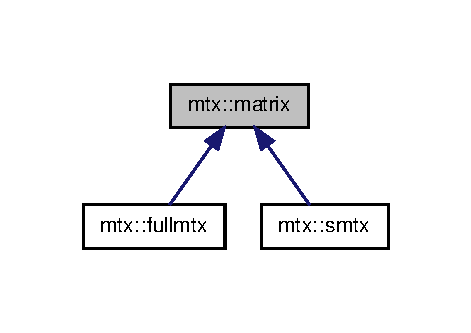
\includegraphics[width=226pt]{structmtx_1_1matrix__inherit__graph}
\end{center}
\end{figure}


\-Collaboration diagram for mtx\-:\-:matrix\-:\nopagebreak
\begin{figure}[H]
\begin{center}
\leavevmode
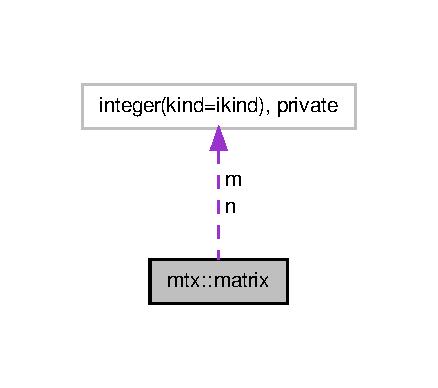
\includegraphics[width=210pt]{structmtx_1_1matrix__coll__graph}
\end{center}
\end{figure}
\subsection*{\-Public \-Member \-Functions}
\begin{DoxyCompactItemize}
\item 
procedure, non\-\_\-overridable \hyperlink{structmtx_1_1matrix_ad43a73f32b347da18f997ce145d6c27c}{getn} =$>$ \hyperlink{classmtx_ab05f486a31448c69570e2144b4010957}{getnmatrix}
\begin{DoxyCompactList}\small\item\em vrati pocet radku \end{DoxyCompactList}\item 
procedure, non\-\_\-overridable \hyperlink{structmtx_1_1matrix_a24f1071ad0cb83094ba23d3027321392}{getm} =$>$ \hyperlink{classmtx_adf266f7c4ef90f6ddc1c654bcad5d149}{getmmatrix}
\begin{DoxyCompactList}\small\item\em vrati pocet sloupcu \end{DoxyCompactList}\item 
procedure(\hyperlink{interfacemtx_1_1ini}{ini}), deferred \hyperlink{structmtx_1_1matrix_a93ca8f74b8962073bdde2cf422abd191}{init}
\begin{DoxyCompactList}\small\item\em inicializace matice \end{DoxyCompactList}\item 
procedure(\hyperlink{interfacemtx_1_1geti}{geti}), deferred \hyperlink{structmtx_1_1matrix_aefbbd3d12a8d6429c183bec463749bda}{get}
\begin{DoxyCompactList}\small\item\em vrati prvek matice \end{DoxyCompactList}\item 
procedure(\hyperlink{interfacemtx_1_1seti}{seti}), deferred, pass \hyperlink{structmtx_1_1matrix_a64b6c3a20c2e85dc715f8cd2f70d6e18}{set}
\begin{DoxyCompactList}\small\item\em nastavi prvek matice \end{DoxyCompactList}\item 
procedure \hyperlink{structmtx_1_1matrix_a99c4dff8cf1c63a968d03474084d0b70}{getrow} =$>$ \hyperlink{classmtx_a46e5fd9002257990ea5c79e1971c8167}{getrowmatrix}
\begin{DoxyCompactList}\small\item\em vybere radek z matice \end{DoxyCompactList}\item 
procedure \hyperlink{structmtx_1_1matrix_af9d60c003f797c73085241d8c38ea792}{getcol} =$>$ \hyperlink{classmtx_abb68e8d5a8216a50b88e5c577b5ad403}{getcolmatrix}
\begin{DoxyCompactList}\small\item\em vybere sloupec z matice \end{DoxyCompactList}\item 
procedure \hyperlink{structmtx_1_1matrix_a4b7b05cc668bbeffed54335122063a03}{print} =$>$ \hyperlink{classmtx_a9b242fed3892da977edee5be16d85bdf}{printmatrix}
\begin{DoxyCompactList}\small\item\em vytiskne matici \end{DoxyCompactList}\item 
procedure \hyperlink{structmtx_1_1matrix_a1eacf25c7fa77ff8766a1ab281f50f19}{dump} =$>$ \hyperlink{classmtx_ae8163b304193b3e31cc36e31113ec9e9}{dumpmatrix}
\begin{DoxyCompactList}\small\item\em dumpne celou strukturu matice \end{DoxyCompactList}\item 
procedure \hyperlink{structmtx_1_1matrix_a085ae99f3dbc3a44fc4eba9471827fd9}{nonzero} =$>$ \hyperlink{classmtx_aac2e9af9cc01d6d2e4c305eb6ba95b7c}{nzmatrix}
\begin{DoxyCompactList}\small\item\em da pocet nenul v matici \end{DoxyCompactList}\item 
procedure, non\-\_\-overridable \hyperlink{structmtx_1_1matrix_a244598586f2b4d2de61eb827c6349485}{spy} =$>$ \hyperlink{classmtx_afba151bbf31e292a36f36279c0d74cf2}{spymatrix}
\begin{DoxyCompactList}\small\item\em textova varianta spy \end{DoxyCompactList}\item 
procedure \hyperlink{structmtx_1_1matrix_acb57be54454a5c1fad3429d8fab32b95}{mul} =$>$ \hyperlink{classmtx_a33216e985c0e2ec6536c2f013f8562ac}{mulmatrix}
\begin{DoxyCompactList}\small\item\em nasobi vektorem \end{DoxyCompactList}\item 
procedure \hyperlink{structmtx_1_1matrix_a54be9493d99d3be7246d31d46e21fd72}{copy} =$>$ \hyperlink{classmtx_add2b7c4a3a806aebca088907544db1e0}{copymatrix}
\begin{DoxyCompactList}\small\item\em udela kopii matice \end{DoxyCompactList}\end{DoxyCompactItemize}
\subsection*{\-Private \-Attributes}
\begin{DoxyCompactItemize}
\item 
integer(kind=ikind), private \hyperlink{structmtx_1_1matrix_a548016c12d711ebbf9c748b9df0c68f8}{n} = 0
\begin{DoxyCompactList}\small\item\em pocet radku \end{DoxyCompactList}\item 
integer(kind=ikind), private \hyperlink{structmtx_1_1matrix_a832ec93e860493148fa67790e44cd594}{m} = 0
\begin{DoxyCompactList}\small\item\em pocet sloupcu \end{DoxyCompactList}\end{DoxyCompactItemize}


\subsection{\-Detailed \-Description}
obecna matice 

\-Definition at line 13 of file mtx.\-f90.



\subsection{\-Member \-Function/\-Subroutine \-Documentation}
\hypertarget{structmtx_1_1matrix_a54be9493d99d3be7246d31d46e21fd72}{\index{mtx\-::matrix@{mtx\-::matrix}!copy@{copy}}
\index{copy@{copy}!mtx::matrix@{mtx\-::matrix}}
\subsubsection[{copy}]{\setlength{\rightskip}{0pt plus 5cm}procedure {\bf mtx\-::matrix\-::copy} (
\begin{DoxyParamCaption}
{}
\end{DoxyParamCaption}
)}}\label{structmtx_1_1matrix_a54be9493d99d3be7246d31d46e21fd72}


udela kopii matice 



\-Definition at line 44 of file mtx.\-f90.

\hypertarget{structmtx_1_1matrix_a1eacf25c7fa77ff8766a1ab281f50f19}{\index{mtx\-::matrix@{mtx\-::matrix}!dump@{dump}}
\index{dump@{dump}!mtx::matrix@{mtx\-::matrix}}
\subsubsection[{dump}]{\setlength{\rightskip}{0pt plus 5cm}procedure {\bf mtx\-::matrix\-::dump} (
\begin{DoxyParamCaption}
{}
\end{DoxyParamCaption}
)}}\label{structmtx_1_1matrix_a1eacf25c7fa77ff8766a1ab281f50f19}


dumpne celou strukturu matice 



\-Reimplemented in \hyperlink{structmtx_1_1smtx_ac7863d852b3115cf545f7ed8356be3fc}{mtx\-::smtx}.



\-Definition at line 36 of file mtx.\-f90.

\hypertarget{structmtx_1_1matrix_aefbbd3d12a8d6429c183bec463749bda}{\index{mtx\-::matrix@{mtx\-::matrix}!get@{get}}
\index{get@{get}!mtx::matrix@{mtx\-::matrix}}
\subsubsection[{get}]{\setlength{\rightskip}{0pt plus 5cm}procedure({\bf geti}), deferred {\bf mtx\-::matrix\-::get} (
\begin{DoxyParamCaption}
{}
\end{DoxyParamCaption}
)}}\label{structmtx_1_1matrix_aefbbd3d12a8d6429c183bec463749bda}


vrati prvek matice 



\-Reimplemented in \hyperlink{structmtx_1_1fullmtx_a2155f93b9fceea289c90e7f01fb505a7}{mtx\-::fullmtx}, and \hyperlink{structmtx_1_1smtx_ad099bd73ffe67c9c01ac973e0cbccf8a}{mtx\-::smtx}.



\-Definition at line 26 of file mtx.\-f90.

\hypertarget{structmtx_1_1matrix_af9d60c003f797c73085241d8c38ea792}{\index{mtx\-::matrix@{mtx\-::matrix}!getcol@{getcol}}
\index{getcol@{getcol}!mtx::matrix@{mtx\-::matrix}}
\subsubsection[{getcol}]{\setlength{\rightskip}{0pt plus 5cm}procedure {\bf mtx\-::matrix\-::getcol} (
\begin{DoxyParamCaption}
{}
\end{DoxyParamCaption}
)}}\label{structmtx_1_1matrix_af9d60c003f797c73085241d8c38ea792}


vybere sloupec z matice 



\-Definition at line 32 of file mtx.\-f90.

\hypertarget{structmtx_1_1matrix_a24f1071ad0cb83094ba23d3027321392}{\index{mtx\-::matrix@{mtx\-::matrix}!getm@{getm}}
\index{getm@{getm}!mtx::matrix@{mtx\-::matrix}}
\subsubsection[{getm}]{\setlength{\rightskip}{0pt plus 5cm}procedure, non\-\_\-overridable {\bf mtx\-::matrix\-::getm} (
\begin{DoxyParamCaption}
{}
\end{DoxyParamCaption}
)}}\label{structmtx_1_1matrix_a24f1071ad0cb83094ba23d3027321392}


vrati pocet sloupcu 



\-Definition at line 22 of file mtx.\-f90.

\hypertarget{structmtx_1_1matrix_ad43a73f32b347da18f997ce145d6c27c}{\index{mtx\-::matrix@{mtx\-::matrix}!getn@{getn}}
\index{getn@{getn}!mtx::matrix@{mtx\-::matrix}}
\subsubsection[{getn}]{\setlength{\rightskip}{0pt plus 5cm}procedure, non\-\_\-overridable {\bf mtx\-::matrix\-::getn} (
\begin{DoxyParamCaption}
{}
\end{DoxyParamCaption}
)}}\label{structmtx_1_1matrix_ad43a73f32b347da18f997ce145d6c27c}


vrati pocet radku 



\-Definition at line 20 of file mtx.\-f90.

\hypertarget{structmtx_1_1matrix_a99c4dff8cf1c63a968d03474084d0b70}{\index{mtx\-::matrix@{mtx\-::matrix}!getrow@{getrow}}
\index{getrow@{getrow}!mtx::matrix@{mtx\-::matrix}}
\subsubsection[{getrow}]{\setlength{\rightskip}{0pt plus 5cm}procedure {\bf mtx\-::matrix\-::getrow} (
\begin{DoxyParamCaption}
{}
\end{DoxyParamCaption}
)}}\label{structmtx_1_1matrix_a99c4dff8cf1c63a968d03474084d0b70}


vybere radek z matice 



\-Definition at line 30 of file mtx.\-f90.

\hypertarget{structmtx_1_1matrix_a93ca8f74b8962073bdde2cf422abd191}{\index{mtx\-::matrix@{mtx\-::matrix}!init@{init}}
\index{init@{init}!mtx::matrix@{mtx\-::matrix}}
\subsubsection[{init}]{\setlength{\rightskip}{0pt plus 5cm}procedure({\bf ini}), deferred {\bf mtx\-::matrix\-::init} (
\begin{DoxyParamCaption}
{}
\end{DoxyParamCaption}
)}}\label{structmtx_1_1matrix_a93ca8f74b8962073bdde2cf422abd191}


inicializace matice 



\-Reimplemented in \hyperlink{structmtx_1_1fullmtx_a61b753f6a76bcfd96fbe82c26bbdce8b}{mtx\-::fullmtx}, and \hyperlink{structmtx_1_1smtx_aad1907a959bc0080ac4b364d6b2a17af}{mtx\-::smtx}.



\-Definition at line 24 of file mtx.\-f90.

\hypertarget{structmtx_1_1matrix_acb57be54454a5c1fad3429d8fab32b95}{\index{mtx\-::matrix@{mtx\-::matrix}!mul@{mul}}
\index{mul@{mul}!mtx::matrix@{mtx\-::matrix}}
\subsubsection[{mul}]{\setlength{\rightskip}{0pt plus 5cm}procedure {\bf mtx\-::matrix\-::mul} (
\begin{DoxyParamCaption}
{}
\end{DoxyParamCaption}
)}}\label{structmtx_1_1matrix_acb57be54454a5c1fad3429d8fab32b95}


nasobi vektorem 



\-Reimplemented in \hyperlink{structmtx_1_1smtx_a799fca1825561095bdb5a3342fb88a21}{mtx\-::smtx}.



\-Definition at line 42 of file mtx.\-f90.

\hypertarget{structmtx_1_1matrix_a085ae99f3dbc3a44fc4eba9471827fd9}{\index{mtx\-::matrix@{mtx\-::matrix}!nonzero@{nonzero}}
\index{nonzero@{nonzero}!mtx::matrix@{mtx\-::matrix}}
\subsubsection[{nonzero}]{\setlength{\rightskip}{0pt plus 5cm}procedure {\bf mtx\-::matrix\-::nonzero} (
\begin{DoxyParamCaption}
{}
\end{DoxyParamCaption}
)}}\label{structmtx_1_1matrix_a085ae99f3dbc3a44fc4eba9471827fd9}


da pocet nenul v matici 



\-Reimplemented in \hyperlink{structmtx_1_1smtx_a6f111e4bbdebc5c728e9064be2164b65}{mtx\-::smtx}.



\-Definition at line 38 of file mtx.\-f90.

\hypertarget{structmtx_1_1matrix_a4b7b05cc668bbeffed54335122063a03}{\index{mtx\-::matrix@{mtx\-::matrix}!print@{print}}
\index{print@{print}!mtx::matrix@{mtx\-::matrix}}
\subsubsection[{print}]{\setlength{\rightskip}{0pt plus 5cm}procedure {\bf mtx\-::matrix\-::print} (
\begin{DoxyParamCaption}
{}
\end{DoxyParamCaption}
)}}\label{structmtx_1_1matrix_a4b7b05cc668bbeffed54335122063a03}


vytiskne matici 



\-Reimplemented in \hyperlink{structmtx_1_1smtx_a3977bc695c6286962667d92261ee7ac2}{mtx\-::smtx}.



\-Definition at line 34 of file mtx.\-f90.

\hypertarget{structmtx_1_1matrix_a64b6c3a20c2e85dc715f8cd2f70d6e18}{\index{mtx\-::matrix@{mtx\-::matrix}!set@{set}}
\index{set@{set}!mtx::matrix@{mtx\-::matrix}}
\subsubsection[{set}]{\setlength{\rightskip}{0pt plus 5cm}procedure({\bf seti}), deferred, pass {\bf mtx\-::matrix\-::set} (
\begin{DoxyParamCaption}
{}
\end{DoxyParamCaption}
)}}\label{structmtx_1_1matrix_a64b6c3a20c2e85dc715f8cd2f70d6e18}


nastavi prvek matice 



\-Reimplemented in \hyperlink{structmtx_1_1fullmtx_ac28edc8d06a554863016c1e369d218c4}{mtx\-::fullmtx}, and \hyperlink{structmtx_1_1smtx_a7cd1a50472a77e6b3894c633e676bd35}{mtx\-::smtx}.



\-Definition at line 28 of file mtx.\-f90.

\hypertarget{structmtx_1_1matrix_a244598586f2b4d2de61eb827c6349485}{\index{mtx\-::matrix@{mtx\-::matrix}!spy@{spy}}
\index{spy@{spy}!mtx::matrix@{mtx\-::matrix}}
\subsubsection[{spy}]{\setlength{\rightskip}{0pt plus 5cm}procedure, non\-\_\-overridable {\bf mtx\-::matrix\-::spy} (
\begin{DoxyParamCaption}
{}
\end{DoxyParamCaption}
)}}\label{structmtx_1_1matrix_a244598586f2b4d2de61eb827c6349485}


textova varianta spy 



\-Definition at line 40 of file mtx.\-f90.



\subsection{\-Member \-Data \-Documentation}
\hypertarget{structmtx_1_1matrix_a832ec93e860493148fa67790e44cd594}{\index{mtx\-::matrix@{mtx\-::matrix}!m@{m}}
\index{m@{m}!mtx::matrix@{mtx\-::matrix}}
\subsubsection[{m}]{\setlength{\rightskip}{0pt plus 5cm}integer(kind=ikind), private {\bf mtx\-::matrix\-::m} = 0\hspace{0.3cm}{\ttfamily  \mbox{[}private\mbox{]}}}}\label{structmtx_1_1matrix_a832ec93e860493148fa67790e44cd594}


pocet sloupcu 



\-Definition at line 17 of file mtx.\-f90.

\hypertarget{structmtx_1_1matrix_a548016c12d711ebbf9c748b9df0c68f8}{\index{mtx\-::matrix@{mtx\-::matrix}!n@{n}}
\index{n@{n}!mtx::matrix@{mtx\-::matrix}}
\subsubsection[{n}]{\setlength{\rightskip}{0pt plus 5cm}integer(kind=ikind), private {\bf mtx\-::matrix\-::n} = 0\hspace{0.3cm}{\ttfamily  \mbox{[}private\mbox{]}}}}\label{structmtx_1_1matrix_a548016c12d711ebbf9c748b9df0c68f8}


pocet radku 



\-Definition at line 15 of file mtx.\-f90.



\-The documentation for this type was generated from the following file\-:\begin{DoxyCompactItemize}
\item 
\hyperlink{mtx_8f90}{mtx.\-f90}\end{DoxyCompactItemize}

\hypertarget{classmtx}{\section{mtx \-Module \-Reference}
\label{classmtx}\index{mtx@{mtx}}
}


module pro matice  


\subsection*{\-Data \-Types}
\begin{DoxyCompactItemize}
\item 
type \hyperlink{structmtx_1_1elemt}{elemt}
\begin{DoxyCompactList}\small\item\em typ pro prvek ridke matice \end{DoxyCompactList}\item 
type \hyperlink{structmtx_1_1fullmtx}{fullmtx}
\begin{DoxyCompactList}\small\item\em plna matice \end{DoxyCompactList}\item 
interface \hyperlink{interfacemtx_1_1geti}{geti}
\begin{DoxyCompactList}\small\item\em interface pro ziskani prvku \end{DoxyCompactList}\item 
interface \hyperlink{interfacemtx_1_1ini}{ini}
\begin{DoxyCompactList}\small\item\em interface pro inicializaci=vymazani matice a resize \end{DoxyCompactList}\item 
type \hyperlink{structmtx_1_1matrix}{matrix}
\begin{DoxyCompactList}\small\item\em obecna matice \end{DoxyCompactList}\item 
interface \hyperlink{interfacemtx_1_1seti}{seti}
\begin{DoxyCompactList}\small\item\em interface pro nastaveni prvku \end{DoxyCompactList}\item 
type \hyperlink{structmtx_1_1smtx}{smtx}
\begin{DoxyCompactList}\small\item\em ridka matice \end{DoxyCompactList}\end{DoxyCompactItemize}
\subsection*{\-Public \-Member \-Functions}
\begin{DoxyCompactItemize}
\item 
pure function \hyperlink{classmtx_ab05f486a31448c69570e2144b4010957}{getnmatrix} (a)
\begin{DoxyCompactList}\small\item\em vrati pocet radku \end{DoxyCompactList}\item 
pure function \hyperlink{classmtx_adf266f7c4ef90f6ddc1c654bcad5d149}{getmmatrix} (a)
\begin{DoxyCompactList}\small\item\em vrati pocet sloupcu \end{DoxyCompactList}\item 
subroutine \hyperlink{classmtx_a46e5fd9002257990ea5c79e1971c8167}{getrowmatrix} (a, i, v, jj, nelem)
\begin{DoxyCompactList}\small\item\em ziska radek z matice -\/ univerzal \end{DoxyCompactList}\item 
subroutine \hyperlink{classmtx_abb68e8d5a8216a50b88e5c577b5ad403}{getcolmatrix} (a, j, v, ii, nelem)
\begin{DoxyCompactList}\small\item\em ziska sloupec z matice \end{DoxyCompactList}\item 
subroutine \hyperlink{classmtx_afba151bbf31e292a36f36279c0d74cf2}{spymatrix} (a)
\begin{DoxyCompactList}\small\item\em napodoba matlabovske spy \end{DoxyCompactList}\item 
subroutine \hyperlink{classmtx_a9b242fed3892da977edee5be16d85bdf}{printmatrix} (a, ncol, width, caption)
\item 
subroutine \hyperlink{classmtx_ae8163b304193b3e31cc36e31113ec9e9}{dumpmatrix} (a)
\begin{DoxyCompactList}\small\item\em zakladni dump \end{DoxyCompactList}\item 
real(kind=rkind) function, \*
dimension(1\-:a\%n) \hyperlink{classmtx_a33216e985c0e2ec6536c2f013f8562ac}{mulmatrix} (a, x, count)
\begin{DoxyCompactList}\small\item\em nasobi matici vektorem \end{DoxyCompactList}\item 
integer(kind=ikind) function \hyperlink{classmtx_ad87ede6266845e9f227148ef4d2d8fc8}{felem} (a, i, j)
\begin{DoxyCompactList}\small\item\em najde prvek v ridke strukture \end{DoxyCompactList}\item 
real(kind=rkind) function \hyperlink{classmtx_ad554ec86f71c2382069ededfe0ce5b8f}{getsp} (a, i, j)
\begin{DoxyCompactList}\small\item\em ziska prvek z ridke matice \end{DoxyCompactList}\item 
subroutine \hyperlink{classmtx_adf89a3418cd4c27c6d678b03bdcb9e12}{setsp} (r, a, i, j)
\begin{DoxyCompactList}\small\item\em nastavi prvek matice, pokud neni tak vlozi \end{DoxyCompactList}\item 
subroutine \hyperlink{classmtx_a4a9f30e7e4915927e3fb4a9eef74c67c}{removesp} (a, i, j, index)
\begin{DoxyCompactList}\small\item\em smazne existujici prvek z ridke matici \end{DoxyCompactList}\item 
subroutine \hyperlink{classmtx_a80356982f18920eb884fc3d702f8ab7d}{initsp} (a, n, m)
\begin{DoxyCompactList}\small\item\em inicializace a vymazani matice \end{DoxyCompactList}\item 
subroutine \hyperlink{classmtx_ac13cd002efa96de601cc9439598ecedb}{sparseprint} (a, ncol, width, caption)
\begin{DoxyCompactList}\small\item\em vytiskne ridkou matici \end{DoxyCompactList}\item 
subroutine \hyperlink{classmtx_ade6ff684a4964e220554d2e1dc9cb846}{sparsedump} (a)
\begin{DoxyCompactList}\small\item\em ridky dump \end{DoxyCompactList}\item 
real(kind=rkind) function, \*
dimension(1\-:a\%n) \hyperlink{classmtx_a05af464426600e96615bc292a3ecfc77}{mulsparse} (a, x, count)
\begin{DoxyCompactList}\small\item\em nasobi matici vektorem \end{DoxyCompactList}\end{DoxyCompactItemize}
\subsection*{\-Private \-Member \-Functions}
\begin{DoxyCompactItemize}
\item 
integer(kind=ikind) function \hyperlink{classmtx_aac2e9af9cc01d6d2e4c305eb6ba95b7c}{nzmatrix} (a)
\begin{DoxyCompactList}\small\item\em vrati pocet nenul v matici -\/ tady n$\ast$m \end{DoxyCompactList}\item 
subroutine \hyperlink{classmtx_add2b7c4a3a806aebca088907544db1e0}{copymatrix} (\-A, \-B)
\begin{DoxyCompactList}\small\item\em zkopiruje matici \end{DoxyCompactList}\item 
real(kind=rkind) function \hyperlink{classmtx_a19fea5b5c69870346797740e80888c31}{getfull} (a, i, j)
\begin{DoxyCompactList}\small\item\em ziska prvek z plne matice \end{DoxyCompactList}\item 
subroutine \hyperlink{classmtx_ad535bdf867ccb7c8e9b27f17609e6517}{setfull} (r, a, i, j)
\begin{DoxyCompactList}\small\item\em vlozi prvek do matice \end{DoxyCompactList}\item 
subroutine \hyperlink{classmtx_a9d997a2261d0627633b50e21779cafeb}{initfull} (a, n, m)
\begin{DoxyCompactList}\small\item\em inicializace plne matice \end{DoxyCompactList}\item 
subroutine \hyperlink{classmtx_acfaae9fe81311d1d0a7c0b57b8db4204}{insertsp} (a, r, i, j)
\begin{DoxyCompactList}\small\item\em prida neexistujici prvek do matice \end{DoxyCompactList}\item 
integer(kind=ikind) function \hyperlink{classmtx_a26863ad7b18a9d30bfc146bc494bcb48}{sparsenz} (a)
\begin{DoxyCompactList}\small\item\em vrati pocet nenul v matici \end{DoxyCompactList}\end{DoxyCompactItemize}


\subsection{\-Detailed \-Description}
module pro matice 

\-Definition at line 7 of file mtx.\-f90.



\subsection{\-Member \-Function/\-Subroutine \-Documentation}
\hypertarget{classmtx_add2b7c4a3a806aebca088907544db1e0}{\index{mtx@{mtx}!copymatrix@{copymatrix}}
\index{copymatrix@{copymatrix}!mtx@{mtx}}
\subsubsection[{copymatrix}]{\setlength{\rightskip}{0pt plus 5cm}subroutine {\bf mtx\-::copymatrix} (
\begin{DoxyParamCaption}
\item[{class({\bf matrix}), intent(inout)}]{\-A, }
\item[{class({\bf matrix}), intent(in)}]{\-B}
\end{DoxyParamCaption}
)\hspace{0.3cm}{\ttfamily  \mbox{[}private\mbox{]}}}}\label{classmtx_add2b7c4a3a806aebca088907544db1e0}


zkopiruje matici 


\begin{DoxyParams}[1]{\-Parameters}
\mbox{\tt in,out}  & {\em \-A} & cil \\
\hline
\mbox{\tt in}  & {\em \-B} & zdroj \\
\hline
\end{DoxyParams}


\-Definition at line 401 of file mtx.\-f90.

\hypertarget{classmtx_ae8163b304193b3e31cc36e31113ec9e9}{\index{mtx@{mtx}!dumpmatrix@{dumpmatrix}}
\index{dumpmatrix@{dumpmatrix}!mtx@{mtx}}
\subsubsection[{dumpmatrix}]{\setlength{\rightskip}{0pt plus 5cm}subroutine {\bf mtx\-::dumpmatrix} (
\begin{DoxyParamCaption}
\item[{class({\bf matrix}), intent(in)}]{a}
\end{DoxyParamCaption}
)}}\label{classmtx_ae8163b304193b3e31cc36e31113ec9e9}


zakladni dump 



\-Definition at line 358 of file mtx.\-f90.

\hypertarget{classmtx_ad87ede6266845e9f227148ef4d2d8fc8}{\index{mtx@{mtx}!felem@{felem}}
\index{felem@{felem}!mtx@{mtx}}
\subsubsection[{felem}]{\setlength{\rightskip}{0pt plus 5cm}integer(kind=ikind) function {\bf mtx\-::felem} (
\begin{DoxyParamCaption}
\item[{class({\bf smtx}), intent(in)}]{a, }
\item[{integer(kind=ikind), intent(in)}]{i, }
\item[{integer(kind=ikind), intent(in)}]{j}
\end{DoxyParamCaption}
)}}\label{classmtx_ad87ede6266845e9f227148ef4d2d8fc8}


najde prvek v ridke strukture 


\begin{DoxyParams}[1]{\-Parameters}
\mbox{\tt in}  & {\em a} & matice \\
\hline
\mbox{\tt in}  & {\em i} & souradnice \\
\hline
\mbox{\tt in}  & {\em j} & souradnice \\
\hline
\end{DoxyParams}


\-Definition at line 468 of file mtx.\-f90.

\hypertarget{classmtx_abb68e8d5a8216a50b88e5c577b5ad403}{\index{mtx@{mtx}!getcolmatrix@{getcolmatrix}}
\index{getcolmatrix@{getcolmatrix}!mtx@{mtx}}
\subsubsection[{getcolmatrix}]{\setlength{\rightskip}{0pt plus 5cm}subroutine {\bf mtx\-::getcolmatrix} (
\begin{DoxyParamCaption}
\item[{class({\bf matrix}), intent(in)}]{a, }
\item[{integer(kind=ikind), intent(in)}]{j, }
\item[{real(kind=rkind), dimension(\-:), intent(inout), allocatable}]{v, }
\item[{integer(kind=ikind), dimension(\-:), intent(inout), allocatable}]{ii, }
\item[{integer(kind=ikind), intent(out)}]{nelem}
\end{DoxyParamCaption}
)}}\label{classmtx_abb68e8d5a8216a50b88e5c577b5ad403}


ziska sloupec z matice 



\-Definition at line 229 of file mtx.\-f90.

\hypertarget{classmtx_a19fea5b5c69870346797740e80888c31}{\index{mtx@{mtx}!getfull@{getfull}}
\index{getfull@{getfull}!mtx@{mtx}}
\subsubsection[{getfull}]{\setlength{\rightskip}{0pt plus 5cm}real(kind=rkind) function {\bf mtx\-::getfull} (
\begin{DoxyParamCaption}
\item[{class({\bf fullmtx}), intent(in)}]{a, }
\item[{integer(kind=ikind), intent(in)}]{i, }
\item[{integer(kind=ikind), intent(in)}]{j}
\end{DoxyParamCaption}
)\hspace{0.3cm}{\ttfamily  \mbox{[}private\mbox{]}}}}\label{classmtx_a19fea5b5c69870346797740e80888c31}


ziska prvek z plne matice 


\begin{DoxyParams}[1]{\-Parameters}
\mbox{\tt in}  & {\em a} & matice \\
\hline
\mbox{\tt in}  & {\em i} & souradnice \\
\hline
\mbox{\tt in}  & {\em j} & souradnice \\
\hline
\end{DoxyParams}


\-Definition at line 423 of file mtx.\-f90.

\hypertarget{classmtx_adf266f7c4ef90f6ddc1c654bcad5d149}{\index{mtx@{mtx}!getmmatrix@{getmmatrix}}
\index{getmmatrix@{getmmatrix}!mtx@{mtx}}
\subsubsection[{getmmatrix}]{\setlength{\rightskip}{0pt plus 5cm}pure function {\bf mtx\-::getmmatrix} (
\begin{DoxyParamCaption}
\item[{class({\bf matrix}), intent(in)}]{a}
\end{DoxyParamCaption}
)}}\label{classmtx_adf266f7c4ef90f6ddc1c654bcad5d149}


vrati pocet sloupcu 


\begin{DoxyParams}[1]{\-Parameters}
\mbox{\tt in}  & {\em a} & matice \\
\hline
\end{DoxyParams}


\-Definition at line 162 of file mtx.\-f90.

\hypertarget{classmtx_ab05f486a31448c69570e2144b4010957}{\index{mtx@{mtx}!getnmatrix@{getnmatrix}}
\index{getnmatrix@{getnmatrix}!mtx@{mtx}}
\subsubsection[{getnmatrix}]{\setlength{\rightskip}{0pt plus 5cm}pure function {\bf mtx\-::getnmatrix} (
\begin{DoxyParamCaption}
\item[{class({\bf matrix}), intent(in)}]{a}
\end{DoxyParamCaption}
)}}\label{classmtx_ab05f486a31448c69570e2144b4010957}


vrati pocet radku 


\begin{DoxyParams}[1]{\-Parameters}
\mbox{\tt in}  & {\em a} & matice \\
\hline
\end{DoxyParams}


\-Definition at line 151 of file mtx.\-f90.

\hypertarget{classmtx_a46e5fd9002257990ea5c79e1971c8167}{\index{mtx@{mtx}!getrowmatrix@{getrowmatrix}}
\index{getrowmatrix@{getrowmatrix}!mtx@{mtx}}
\subsubsection[{getrowmatrix}]{\setlength{\rightskip}{0pt plus 5cm}subroutine {\bf mtx\-::getrowmatrix} (
\begin{DoxyParamCaption}
\item[{class({\bf matrix}), intent(in)}]{a, }
\item[{integer(kind=ikind)}]{i, }
\item[{real(kind=rkind), dimension(\-:), intent(inout), allocatable}]{v, }
\item[{integer(kind=ikind), dimension(\-:), intent(inout), allocatable}]{jj, }
\item[{integer(kind=ikind), intent(out)}]{nelem}
\end{DoxyParamCaption}
)}}\label{classmtx_a46e5fd9002257990ea5c79e1971c8167}


ziska radek z matice -\/ univerzal 

vrati jen nenulove prvky z radku, v pripade potreby prealokuje prostor 
\begin{DoxyParams}[1]{\-Parameters}
\mbox{\tt in}  & {\em a} & matice \\
\hline
 & {\em i} & pozadovany radek \\
\hline
\mbox{\tt in,out}  & {\em v} & nenulove hodnoty z radku \\
\hline
\mbox{\tt in,out}  & {\em jj} & sloupcove indexy nenulovych prvku radku \\
\hline
\mbox{\tt out}  & {\em nelem} & pocet nenulovych prvku v radku \\
\hline
\end{DoxyParams}


\-Definition at line 175 of file mtx.\-f90.

\hypertarget{classmtx_ad554ec86f71c2382069ededfe0ce5b8f}{\index{mtx@{mtx}!getsp@{getsp}}
\index{getsp@{getsp}!mtx@{mtx}}
\subsubsection[{getsp}]{\setlength{\rightskip}{0pt plus 5cm}real(kind=rkind) function {\bf mtx\-::getsp} (
\begin{DoxyParamCaption}
\item[{class({\bf smtx}), intent(in)}]{a, }
\item[{integer(kind=ikind), intent(in)}]{i, }
\item[{integer(kind=ikind), intent(in)}]{j}
\end{DoxyParamCaption}
)}}\label{classmtx_ad554ec86f71c2382069ededfe0ce5b8f}


ziska prvek z ridke matice 


\begin{DoxyParams}[1]{\-Parameters}
\mbox{\tt in}  & {\em a} & matice \\
\hline
\mbox{\tt in}  & {\em i} & souradnice \\
\hline
\mbox{\tt in}  & {\em j} & souradnice \\
\hline
\end{DoxyParams}


\-Definition at line 492 of file mtx.\-f90.

\hypertarget{classmtx_a9d997a2261d0627633b50e21779cafeb}{\index{mtx@{mtx}!initfull@{initfull}}
\index{initfull@{initfull}!mtx@{mtx}}
\subsubsection[{initfull}]{\setlength{\rightskip}{0pt plus 5cm}subroutine {\bf mtx\-::initfull} (
\begin{DoxyParamCaption}
\item[{class({\bf fullmtx}), intent(inout)}]{a, }
\item[{integer(kind=ikind), intent(in)}]{n, }
\item[{integer(kind=ikind), intent(in)}]{m}
\end{DoxyParamCaption}
)\hspace{0.3cm}{\ttfamily  \mbox{[}private\mbox{]}}}}\label{classmtx_a9d997a2261d0627633b50e21779cafeb}


inicializace plne matice 


\begin{DoxyParams}[1]{\-Parameters}
\mbox{\tt in,out}  & {\em a} & matice \\
\hline
\mbox{\tt in}  & {\em n} & rozmery matice \\
\hline
\mbox{\tt in}  & {\em m} & rozmery matice \\
\hline
\end{DoxyParams}


\-Definition at line 449 of file mtx.\-f90.

\hypertarget{classmtx_a80356982f18920eb884fc3d702f8ab7d}{\index{mtx@{mtx}!initsp@{initsp}}
\index{initsp@{initsp}!mtx@{mtx}}
\subsubsection[{initsp}]{\setlength{\rightskip}{0pt plus 5cm}subroutine {\bf mtx\-::initsp} (
\begin{DoxyParamCaption}
\item[{class({\bf smtx}), intent(inout)}]{a, }
\item[{integer(kind=ikind), intent(in)}]{n, }
\item[{integer(kind=ikind), intent(in)}]{m}
\end{DoxyParamCaption}
)}}\label{classmtx_a80356982f18920eb884fc3d702f8ab7d}


inicializace a vymazani matice 


\begin{DoxyParams}[1]{\-Parameters}
\mbox{\tt in,out}  & {\em a} & matice \\
\hline
\mbox{\tt in}  & {\em n} & rozmery \\
\hline
\mbox{\tt in}  & {\em m} & rozmery \\
\hline
\end{DoxyParams}


\-Definition at line 709 of file mtx.\-f90.

\hypertarget{classmtx_acfaae9fe81311d1d0a7c0b57b8db4204}{\index{mtx@{mtx}!insertsp@{insertsp}}
\index{insertsp@{insertsp}!mtx@{mtx}}
\subsubsection[{insertsp}]{\setlength{\rightskip}{0pt plus 5cm}subroutine {\bf mtx\-::insertsp} (
\begin{DoxyParamCaption}
\item[{class({\bf smtx}), intent(inout)}]{a, }
\item[{real(kind=rkind), intent(in)}]{r, }
\item[{integer(kind=ikind), intent(in)}]{i, }
\item[{integer(kind=ikind), intent(in)}]{j}
\end{DoxyParamCaption}
)\hspace{0.3cm}{\ttfamily  \mbox{[}private\mbox{]}}}}\label{classmtx_acfaae9fe81311d1d0a7c0b57b8db4204}


prida neexistujici prvek do matice 


\begin{DoxyParams}[1]{\-Parameters}
\mbox{\tt in,out}  & {\em a} & matice \\
\hline
\mbox{\tt in}  & {\em r} & hodnota \\
\hline
\mbox{\tt in}  & {\em i} & souradnice \\
\hline
\mbox{\tt in}  & {\em j} & souradnice \\
\hline
\end{DoxyParams}


\-Definition at line 532 of file mtx.\-f90.

\hypertarget{classmtx_a33216e985c0e2ec6536c2f013f8562ac}{\index{mtx@{mtx}!mulmatrix@{mulmatrix}}
\index{mulmatrix@{mulmatrix}!mtx@{mtx}}
\subsubsection[{mulmatrix}]{\setlength{\rightskip}{0pt plus 5cm}real(kind=rkind) function, dimension(1\-:a\%n) {\bf mtx\-::mulmatrix} (
\begin{DoxyParamCaption}
\item[{class({\bf matrix}), intent(in)}]{a, }
\item[{real(kind=rkind), dimension(\-:), intent(in)}]{x, }
\item[{type(tcount), intent(inout), optional}]{count}
\end{DoxyParamCaption}
)}}\label{classmtx_a33216e985c0e2ec6536c2f013f8562ac}


nasobi matici vektorem 


\begin{DoxyParams}[1]{\-Parameters}
\mbox{\tt in}  & {\em a} & matice \\
\hline
\mbox{\tt in}  & {\em x} & vektor \\
\hline
\mbox{\tt in,out}  & {\em count} & pocet operaci \\
\hline
\end{DoxyParams}


\-Definition at line 376 of file mtx.\-f90.

\hypertarget{classmtx_a05af464426600e96615bc292a3ecfc77}{\index{mtx@{mtx}!mulsparse@{mulsparse}}
\index{mulsparse@{mulsparse}!mtx@{mtx}}
\subsubsection[{mulsparse}]{\setlength{\rightskip}{0pt plus 5cm}real(kind=rkind) function, dimension(1\-:a\%n) {\bf mtx\-::mulsparse} (
\begin{DoxyParamCaption}
\item[{class({\bf smtx}), intent(in)}]{a, }
\item[{real(kind=rkind), dimension(\-:), intent(in)}]{x, }
\item[{type(tcount), intent(inout), optional}]{count}
\end{DoxyParamCaption}
)}}\label{classmtx_a05af464426600e96615bc292a3ecfc77}


nasobi matici vektorem 


\begin{DoxyParams}[1]{\-Parameters}
\mbox{\tt in}  & {\em a} & matice \\
\hline
\mbox{\tt in}  & {\em x} & vektor \\
\hline
\mbox{\tt in,out}  & {\em count} & pocet operaci \\
\hline
\end{DoxyParams}


\-Definition at line 817 of file mtx.\-f90.

\hypertarget{classmtx_aac2e9af9cc01d6d2e4c305eb6ba95b7c}{\index{mtx@{mtx}!nzmatrix@{nzmatrix}}
\index{nzmatrix@{nzmatrix}!mtx@{mtx}}
\subsubsection[{nzmatrix}]{\setlength{\rightskip}{0pt plus 5cm}integer(kind=ikind) function {\bf mtx\-::nzmatrix} (
\begin{DoxyParamCaption}
\item[{class({\bf matrix}), intent(in)}]{a}
\end{DoxyParamCaption}
)\hspace{0.3cm}{\ttfamily  \mbox{[}private\mbox{]}}}}\label{classmtx_aac2e9af9cc01d6d2e4c305eb6ba95b7c}


vrati pocet nenul v matici -\/ tady n$\ast$m 



\-Definition at line 366 of file mtx.\-f90.

\hypertarget{classmtx_a9b242fed3892da977edee5be16d85bdf}{\index{mtx@{mtx}!printmatrix@{printmatrix}}
\index{printmatrix@{printmatrix}!mtx@{mtx}}
\subsubsection[{printmatrix}]{\setlength{\rightskip}{0pt plus 5cm}subroutine {\bf mtx\-::printmatrix} (
\begin{DoxyParamCaption}
\item[{class({\bf matrix}), intent(in)}]{a, }
\item[{integer(kind=ikind), intent(in), optional}]{ncol, }
\item[{integer(kind=ikind), intent(in), optional}]{width, }
\item[{character(len=$\ast$), intent(in), optional}]{caption}
\end{DoxyParamCaption}
)}}\label{classmtx_a9b242fed3892da977edee5be16d85bdf}


\-Definition at line 303 of file mtx.\-f90.

\hypertarget{classmtx_a4a9f30e7e4915927e3fb4a9eef74c67c}{\index{mtx@{mtx}!removesp@{removesp}}
\index{removesp@{removesp}!mtx@{mtx}}
\subsubsection[{removesp}]{\setlength{\rightskip}{0pt plus 5cm}subroutine {\bf mtx\-::removesp} (
\begin{DoxyParamCaption}
\item[{class({\bf smtx}), intent(inout)}]{a, }
\item[{integer(kind=ikind), intent(in)}]{i, }
\item[{integer(kind=ikind), intent(in)}]{j, }
\item[{integer(kind=ikind), intent(in)}]{index}
\end{DoxyParamCaption}
)}}\label{classmtx_a4a9f30e7e4915927e3fb4a9eef74c67c}


smazne existujici prvek z ridke matici 


\begin{DoxyParams}[1]{\-Parameters}
\mbox{\tt in,out}  & {\em a} & matice \\
\hline
\mbox{\tt in}  & {\em i} & souradnice a pozice \\
\hline
\mbox{\tt in}  & {\em j} & souradnice a pozice \\
\hline
\mbox{\tt in}  & {\em index} & souradnice a pozice \\
\hline
\end{DoxyParams}


\-Definition at line 641 of file mtx.\-f90.

\hypertarget{classmtx_ad535bdf867ccb7c8e9b27f17609e6517}{\index{mtx@{mtx}!setfull@{setfull}}
\index{setfull@{setfull}!mtx@{mtx}}
\subsubsection[{setfull}]{\setlength{\rightskip}{0pt plus 5cm}subroutine {\bf mtx\-::setfull} (
\begin{DoxyParamCaption}
\item[{real(kind=rkind), intent(in)}]{r, }
\item[{class({\bf fullmtx}), intent(inout)}]{a, }
\item[{integer(kind=ikind), intent(in)}]{i, }
\item[{integer(kind=ikind), intent(in)}]{j}
\end{DoxyParamCaption}
)\hspace{0.3cm}{\ttfamily  \mbox{[}private\mbox{]}}}}\label{classmtx_ad535bdf867ccb7c8e9b27f17609e6517}


vlozi prvek do matice 


\begin{DoxyParams}[1]{\-Parameters}
\mbox{\tt in}  & {\em r} & hodnota \\
\hline
\mbox{\tt in,out}  & {\em a} & matice \\
\hline
\mbox{\tt in}  & {\em i} & souradnice \\
\hline
\mbox{\tt in}  & {\em j} & souradnice \\
\hline
\end{DoxyParams}


\-Definition at line 435 of file mtx.\-f90.

\hypertarget{classmtx_adf89a3418cd4c27c6d678b03bdcb9e12}{\index{mtx@{mtx}!setsp@{setsp}}
\index{setsp@{setsp}!mtx@{mtx}}
\subsubsection[{setsp}]{\setlength{\rightskip}{0pt plus 5cm}subroutine {\bf mtx\-::setsp} (
\begin{DoxyParamCaption}
\item[{real(kind=rkind), intent(in)}]{r, }
\item[{class({\bf smtx}), intent(inout)}]{a, }
\item[{integer(kind=ikind), intent(in)}]{i, }
\item[{integer(kind=ikind), intent(in)}]{j}
\end{DoxyParamCaption}
)}}\label{classmtx_adf89a3418cd4c27c6d678b03bdcb9e12}


nastavi prvek matice, pokud neni tak vlozi 


\begin{DoxyParams}[1]{\-Parameters}
\mbox{\tt in}  & {\em r} & hodnota \\
\hline
\mbox{\tt in,out}  & {\em a} & matice \\
\hline
\mbox{\tt in}  & {\em i} & souradnice \\
\hline
\mbox{\tt in}  & {\em j} & souradnice \\
\hline
\end{DoxyParams}


\-Definition at line 506 of file mtx.\-f90.

\hypertarget{classmtx_ade6ff684a4964e220554d2e1dc9cb846}{\index{mtx@{mtx}!sparsedump@{sparsedump}}
\index{sparsedump@{sparsedump}!mtx@{mtx}}
\subsubsection[{sparsedump}]{\setlength{\rightskip}{0pt plus 5cm}subroutine {\bf mtx\-::sparsedump} (
\begin{DoxyParamCaption}
\item[{class({\bf smtx}), intent(in)}]{a}
\end{DoxyParamCaption}
)}}\label{classmtx_ade6ff684a4964e220554d2e1dc9cb846}


ridky dump 



\-Definition at line 780 of file mtx.\-f90.

\hypertarget{classmtx_a26863ad7b18a9d30bfc146bc494bcb48}{\index{mtx@{mtx}!sparsenz@{sparsenz}}
\index{sparsenz@{sparsenz}!mtx@{mtx}}
\subsubsection[{sparsenz}]{\setlength{\rightskip}{0pt plus 5cm}integer(kind=ikind) function {\bf mtx\-::sparsenz} (
\begin{DoxyParamCaption}
\item[{class({\bf smtx}), intent(in)}]{a}
\end{DoxyParamCaption}
)\hspace{0.3cm}{\ttfamily  \mbox{[}private\mbox{]}}}}\label{classmtx_a26863ad7b18a9d30bfc146bc494bcb48}


vrati pocet nenul v matici 


\begin{DoxyParams}[1]{\-Parameters}
\mbox{\tt in}  & {\em a} & matice \\
\hline
\end{DoxyParams}


\-Definition at line 806 of file mtx.\-f90.

\hypertarget{classmtx_ac13cd002efa96de601cc9439598ecedb}{\index{mtx@{mtx}!sparseprint@{sparseprint}}
\index{sparseprint@{sparseprint}!mtx@{mtx}}
\subsubsection[{sparseprint}]{\setlength{\rightskip}{0pt plus 5cm}subroutine {\bf mtx\-::sparseprint} (
\begin{DoxyParamCaption}
\item[{class({\bf smtx}), intent(in)}]{a, }
\item[{integer(kind=ikind), intent(in), optional}]{ncol, }
\item[{integer(kind=ikind), intent(in), optional}]{width, }
\item[{character(len=$\ast$), intent(in), optional}]{caption}
\end{DoxyParamCaption}
)}}\label{classmtx_ac13cd002efa96de601cc9439598ecedb}


vytiskne ridkou matici 


\begin{DoxyParams}[1]{\-Parameters}
\mbox{\tt in}  & {\em a} & matice \\
\hline
\mbox{\tt in}  & {\em ncol} & pocet sloupci tisku \\
\hline
\mbox{\tt in}  & {\em width} & sirka cisla \\
\hline
\mbox{\tt in}  & {\em caption} & nadpis \\
\hline
\end{DoxyParams}


\-Definition at line 728 of file mtx.\-f90.

\hypertarget{classmtx_afba151bbf31e292a36f36279c0d74cf2}{\index{mtx@{mtx}!spymatrix@{spymatrix}}
\index{spymatrix@{spymatrix}!mtx@{mtx}}
\subsubsection[{spymatrix}]{\setlength{\rightskip}{0pt plus 5cm}subroutine {\bf mtx\-::spymatrix} (
\begin{DoxyParamCaption}
\item[{class({\bf matrix}), intent(in)}]{a}
\end{DoxyParamCaption}
)}}\label{classmtx_afba151bbf31e292a36f36279c0d74cf2}


napodoba matlabovske spy 


\begin{DoxyParams}[1]{\-Parameters}
\mbox{\tt in}  & {\em a} & matice \\
\hline
\end{DoxyParams}


\-Definition at line 278 of file mtx.\-f90.



\-The documentation for this module was generated from the following file\-:\begin{DoxyCompactItemize}
\item 
\hyperlink{mtx_8f90}{mtx.\-f90}\end{DoxyCompactItemize}

\hypertarget{interfacemtx_1_1seti}{\section{mtx\-:\-:seti \-Interface \-Reference}
\label{interfacemtx_1_1seti}\index{mtx\-::seti@{mtx\-::seti}}
}


interface pro nastaveni prvku  


\subsection*{\-Private \-Member \-Functions}
\begin{DoxyCompactItemize}
\item 
subroutine \hyperlink{interfacemtx_1_1seti_a9fdf84fcf3ea0273201d44bf9e713480}{seti} (r, a, i, j)
\end{DoxyCompactItemize}


\subsection{\-Detailed \-Description}
interface pro nastaveni prvku 

rutina pro nastaveni prvku 

\-Definition at line 67 of file mtx.\-f90.



\subsection{\-Constructor \& \-Destructor \-Documentation}
\hypertarget{interfacemtx_1_1seti_a9fdf84fcf3ea0273201d44bf9e713480}{\index{mtx\-::seti@{mtx\-::seti}!seti@{seti}}
\index{seti@{seti}!mtx::seti@{mtx\-::seti}}
\subsubsection[{seti}]{\setlength{\rightskip}{0pt plus 5cm}subroutine {\bf mtx\-::seti\-::seti} (
\begin{DoxyParamCaption}
\item[{real(kind=rkind), intent(in)}]{r, }
\item[{class({\bf matrix}), intent(inout)}]{a, }
\item[{integer(kind=ikind), intent(in)}]{i, }
\item[{integer(kind=ikind), intent(in)}]{j}
\end{DoxyParamCaption}
)\hspace{0.3cm}{\ttfamily  \mbox{[}private\mbox{]}}}}\label{interfacemtx_1_1seti_a9fdf84fcf3ea0273201d44bf9e713480}

\begin{DoxyParams}[1]{\-Parameters}
\mbox{\tt in,out}  & {\em a} & matice\\
\hline
\mbox{\tt in}  & {\em i} & souradnice\\
\hline
\mbox{\tt in}  & {\em j} & souradnice\\
\hline
\mbox{\tt in}  & {\em r} & hodnota \\
\hline
\end{DoxyParams}


\-Definition at line 67 of file mtx.\-f90.



\-The documentation for this interface was generated from the following file\-:\begin{DoxyCompactItemize}
\item 
\hyperlink{mtx_8f90}{mtx.\-f90}\end{DoxyCompactItemize}

\hypertarget{structmtx_1_1smtx}{\section{mtx\-:\-:smtx \-Type \-Reference}
\label{structmtx_1_1smtx}\index{mtx\-::smtx@{mtx\-::smtx}}
}


ridka matice  




\-Inheritance diagram for mtx\-:\-:smtx\-:\nopagebreak
\begin{figure}[H]
\begin{center}
\leavevmode
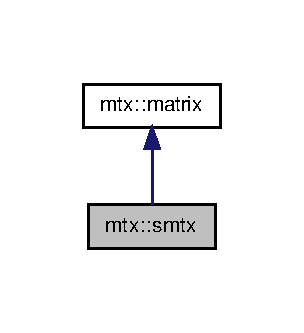
\includegraphics[width=146pt]{structmtx_1_1smtx__inherit__graph}
\end{center}
\end{figure}


\-Collaboration diagram for mtx\-:\-:smtx\-:\nopagebreak
\begin{figure}[H]
\begin{center}
\leavevmode
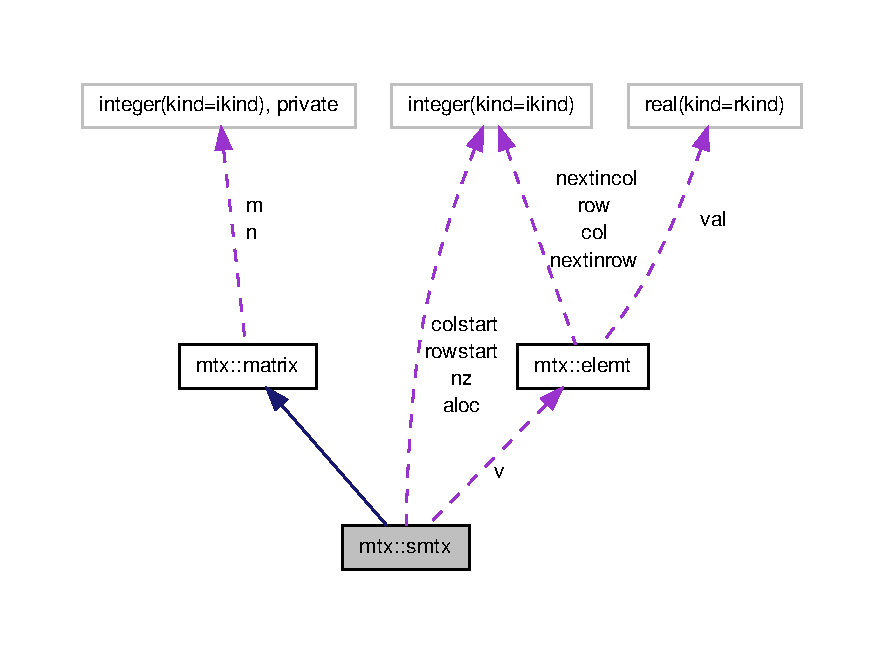
\includegraphics[width=350pt]{structmtx_1_1smtx__coll__graph}
\end{center}
\end{figure}
\subsection*{\-Public \-Member \-Functions}
\begin{DoxyCompactItemize}
\item 
procedure \hyperlink{structmtx_1_1smtx_aad1907a959bc0080ac4b364d6b2a17af}{init} =$>$ \hyperlink{classmtx_a80356982f18920eb884fc3d702f8ab7d}{initsp}
\begin{DoxyCompactList}\small\item\em inicializace matice \end{DoxyCompactList}\item 
procedure \hyperlink{structmtx_1_1smtx_ad099bd73ffe67c9c01ac973e0cbccf8a}{get} =$>$ \hyperlink{classmtx_ad554ec86f71c2382069ededfe0ce5b8f}{getsp}
\begin{DoxyCompactList}\small\item\em vrati prvek matice \end{DoxyCompactList}\item 
procedure, pass(a) \hyperlink{structmtx_1_1smtx_a7cd1a50472a77e6b3894c633e676bd35}{set} =$>$ \hyperlink{classmtx_adf89a3418cd4c27c6d678b03bdcb9e12}{setsp}
\begin{DoxyCompactList}\small\item\em nastavi prvek matice \end{DoxyCompactList}\item 
procedure \hyperlink{structmtx_1_1smtx_a3977bc695c6286962667d92261ee7ac2}{print} =$>$ \hyperlink{classmtx_ac13cd002efa96de601cc9439598ecedb}{sparseprint}
\begin{DoxyCompactList}\small\item\em vytiskne matici \end{DoxyCompactList}\item 
procedure \hyperlink{structmtx_1_1smtx_ac7863d852b3115cf545f7ed8356be3fc}{dump} =$>$ \hyperlink{classmtx_ade6ff684a4964e220554d2e1dc9cb846}{sparsedump}
\begin{DoxyCompactList}\small\item\em dumpne celou strukturu matice \end{DoxyCompactList}\item 
procedure \hyperlink{structmtx_1_1smtx_a6f111e4bbdebc5c728e9064be2164b65}{nonzero} =$>$ \hyperlink{classmtx_a26863ad7b18a9d30bfc146bc494bcb48}{sparsenz}
\begin{DoxyCompactList}\small\item\em da pocet nenul v matici \end{DoxyCompactList}\item 
procedure \hyperlink{structmtx_1_1smtx_a799fca1825561095bdb5a3342fb88a21}{mul} =$>$ \hyperlink{classmtx_a05af464426600e96615bc292a3ecfc77}{mulsparse}
\begin{DoxyCompactList}\small\item\em nasobi vektorem \end{DoxyCompactList}\item 
procedure, non\-\_\-overridable \hyperlink{structmtx_1_1matrix_ad43a73f32b347da18f997ce145d6c27c}{getn} =$>$ \hyperlink{classmtx_ab05f486a31448c69570e2144b4010957}{getnmatrix}
\begin{DoxyCompactList}\small\item\em vrati pocet radku \end{DoxyCompactList}\item 
procedure, non\-\_\-overridable \hyperlink{structmtx_1_1matrix_a24f1071ad0cb83094ba23d3027321392}{getm} =$>$ \hyperlink{classmtx_adf266f7c4ef90f6ddc1c654bcad5d149}{getmmatrix}
\begin{DoxyCompactList}\small\item\em vrati pocet sloupcu \end{DoxyCompactList}\item 
procedure \hyperlink{structmtx_1_1matrix_a99c4dff8cf1c63a968d03474084d0b70}{getrow} =$>$ \hyperlink{classmtx_a46e5fd9002257990ea5c79e1971c8167}{getrowmatrix}
\begin{DoxyCompactList}\small\item\em vybere radek z matice \end{DoxyCompactList}\item 
procedure \hyperlink{structmtx_1_1matrix_af9d60c003f797c73085241d8c38ea792}{getcol} =$>$ \hyperlink{classmtx_abb68e8d5a8216a50b88e5c577b5ad403}{getcolmatrix}
\begin{DoxyCompactList}\small\item\em vybere sloupec z matice \end{DoxyCompactList}\item 
procedure, non\-\_\-overridable \hyperlink{structmtx_1_1matrix_a244598586f2b4d2de61eb827c6349485}{spy} =$>$ \hyperlink{classmtx_afba151bbf31e292a36f36279c0d74cf2}{spymatrix}
\begin{DoxyCompactList}\small\item\em textova varianta spy \end{DoxyCompactList}\item 
procedure \hyperlink{structmtx_1_1matrix_a54be9493d99d3be7246d31d46e21fd72}{copy} =$>$ \hyperlink{classmtx_add2b7c4a3a806aebca088907544db1e0}{copymatrix}
\begin{DoxyCompactList}\small\item\em udela kopii matice \end{DoxyCompactList}\end{DoxyCompactItemize}
\subsection*{\-Private \-Member \-Functions}
\begin{DoxyCompactItemize}
\item 
procedure, private \hyperlink{structmtx_1_1smtx_a42927bac81aa7477787679e5f02ac163}{findelem} =$>$ \hyperlink{classmtx_ad87ede6266845e9f227148ef4d2d8fc8}{felem}
\item 
procedure, private \hyperlink{structmtx_1_1smtx_aa5679cefb1f2b55bf371908580d89dcf}{insert} =$>$ \hyperlink{classmtx_acfaae9fe81311d1d0a7c0b57b8db4204}{insertsp}
\item 
procedure, private \hyperlink{structmtx_1_1smtx_a050bacd00a53420fd9eabc8a0ef39b04}{remove} =$>$ \hyperlink{classmtx_a4a9f30e7e4915927e3fb4a9eef74c67c}{removesp}
\end{DoxyCompactItemize}
\subsection*{\-Private \-Attributes}
\begin{DoxyCompactItemize}
\item 
integer(kind=ikind), private \hyperlink{structmtx_1_1smtx_afa772e98ed5d92de7af52fa3fd90ab02}{nz} = 0
\begin{DoxyCompactList}\small\item\em pocet nenul \end{DoxyCompactList}\item 
integer(kind=ikind), private \hyperlink{structmtx_1_1smtx_acea14dde1b53852c39053ef8c417a6fc}{aloc} = 0
\begin{DoxyCompactList}\small\item\em pocet alokovanych prvku \end{DoxyCompactList}\item 
type(\hyperlink{structmtx_1_1elemt}{elemt}), dimension(\-:), \*
allocatable, private \hyperlink{structmtx_1_1smtx_aefb573912d9722d432a04e74fad75ba9}{v}
\begin{DoxyCompactList}\small\item\em hodnoty prvku \end{DoxyCompactList}\item 
integer(kind=ikind), dimension(\-:), \*
allocatable, private \hyperlink{structmtx_1_1smtx_a363f8a38834bc21f7db7a79f171e72d0}{rowstart}
\begin{DoxyCompactList}\small\item\em zacatky radku -\/ pokud prazdny = -\/1 \end{DoxyCompactList}\item 
integer(kind=ikind), dimension(\-:), \*
allocatable, private \hyperlink{structmtx_1_1smtx_af03dd1dc7a8fe0743a84e2cce99563ff}{colstart}
\begin{DoxyCompactList}\small\item\em zacatky sloupcu -\/ pokud prazdny = -\/1 \end{DoxyCompactList}\end{DoxyCompactItemize}


\subsection{\-Detailed \-Description}
ridka matice 

\-Definition at line 119 of file mtx.\-f90.



\subsection{\-Member \-Function/\-Subroutine \-Documentation}
\hypertarget{structmtx_1_1matrix_a54be9493d99d3be7246d31d46e21fd72}{\index{mtx\-::smtx@{mtx\-::smtx}!copy@{copy}}
\index{copy@{copy}!mtx::smtx@{mtx\-::smtx}}
\subsubsection[{copy}]{\setlength{\rightskip}{0pt plus 5cm}procedure {\bf mtx\-::matrix\-::copy} (
\begin{DoxyParamCaption}
{}
\end{DoxyParamCaption}
)\hspace{0.3cm}{\ttfamily  \mbox{[}inherited\mbox{]}}}}\label{structmtx_1_1matrix_a54be9493d99d3be7246d31d46e21fd72}


udela kopii matice 



\-Definition at line 44 of file mtx.\-f90.

\hypertarget{structmtx_1_1smtx_ac7863d852b3115cf545f7ed8356be3fc}{\index{mtx\-::smtx@{mtx\-::smtx}!dump@{dump}}
\index{dump@{dump}!mtx::smtx@{mtx\-::smtx}}
\subsubsection[{dump}]{\setlength{\rightskip}{0pt plus 5cm}procedure {\bf mtx\-::smtx\-::dump} (
\begin{DoxyParamCaption}
{}
\end{DoxyParamCaption}
)}}\label{structmtx_1_1smtx_ac7863d852b3115cf545f7ed8356be3fc}


dumpne celou strukturu matice 



\-Reimplemented from \hyperlink{structmtx_1_1matrix_a1eacf25c7fa77ff8766a1ab281f50f19}{mtx\-::matrix}.



\-Definition at line 135 of file mtx.\-f90.

\hypertarget{structmtx_1_1smtx_a42927bac81aa7477787679e5f02ac163}{\index{mtx\-::smtx@{mtx\-::smtx}!findelem@{findelem}}
\index{findelem@{findelem}!mtx::smtx@{mtx\-::smtx}}
\subsubsection[{findelem}]{\setlength{\rightskip}{0pt plus 5cm}procedure, private {\bf mtx\-::smtx\-::findelem} (
\begin{DoxyParamCaption}
{}
\end{DoxyParamCaption}
)\hspace{0.3cm}{\ttfamily  \mbox{[}private\mbox{]}}}}\label{structmtx_1_1smtx_a42927bac81aa7477787679e5f02ac163}


\-Definition at line 138 of file mtx.\-f90.

\hypertarget{structmtx_1_1smtx_ad099bd73ffe67c9c01ac973e0cbccf8a}{\index{mtx\-::smtx@{mtx\-::smtx}!get@{get}}
\index{get@{get}!mtx::smtx@{mtx\-::smtx}}
\subsubsection[{get}]{\setlength{\rightskip}{0pt plus 5cm}procedure {\bf mtx\-::smtx\-::get} (
\begin{DoxyParamCaption}
{}
\end{DoxyParamCaption}
)}}\label{structmtx_1_1smtx_ad099bd73ffe67c9c01ac973e0cbccf8a}


vrati prvek matice 



\-Reimplemented from \hyperlink{structmtx_1_1matrix_aefbbd3d12a8d6429c183bec463749bda}{mtx\-::matrix}.



\-Definition at line 132 of file mtx.\-f90.

\hypertarget{structmtx_1_1matrix_af9d60c003f797c73085241d8c38ea792}{\index{mtx\-::smtx@{mtx\-::smtx}!getcol@{getcol}}
\index{getcol@{getcol}!mtx::smtx@{mtx\-::smtx}}
\subsubsection[{getcol}]{\setlength{\rightskip}{0pt plus 5cm}procedure {\bf mtx\-::matrix\-::getcol} (
\begin{DoxyParamCaption}
{}
\end{DoxyParamCaption}
)\hspace{0.3cm}{\ttfamily  \mbox{[}inherited\mbox{]}}}}\label{structmtx_1_1matrix_af9d60c003f797c73085241d8c38ea792}


vybere sloupec z matice 



\-Definition at line 32 of file mtx.\-f90.

\hypertarget{structmtx_1_1matrix_a24f1071ad0cb83094ba23d3027321392}{\index{mtx\-::smtx@{mtx\-::smtx}!getm@{getm}}
\index{getm@{getm}!mtx::smtx@{mtx\-::smtx}}
\subsubsection[{getm}]{\setlength{\rightskip}{0pt plus 5cm}procedure, non\-\_\-overridable {\bf mtx\-::matrix\-::getm} (
\begin{DoxyParamCaption}
{}
\end{DoxyParamCaption}
)\hspace{0.3cm}{\ttfamily  \mbox{[}inherited\mbox{]}}}}\label{structmtx_1_1matrix_a24f1071ad0cb83094ba23d3027321392}


vrati pocet sloupcu 



\-Definition at line 22 of file mtx.\-f90.

\hypertarget{structmtx_1_1matrix_ad43a73f32b347da18f997ce145d6c27c}{\index{mtx\-::smtx@{mtx\-::smtx}!getn@{getn}}
\index{getn@{getn}!mtx::smtx@{mtx\-::smtx}}
\subsubsection[{getn}]{\setlength{\rightskip}{0pt plus 5cm}procedure, non\-\_\-overridable {\bf mtx\-::matrix\-::getn} (
\begin{DoxyParamCaption}
{}
\end{DoxyParamCaption}
)\hspace{0.3cm}{\ttfamily  \mbox{[}inherited\mbox{]}}}}\label{structmtx_1_1matrix_ad43a73f32b347da18f997ce145d6c27c}


vrati pocet radku 



\-Definition at line 20 of file mtx.\-f90.

\hypertarget{structmtx_1_1matrix_a99c4dff8cf1c63a968d03474084d0b70}{\index{mtx\-::smtx@{mtx\-::smtx}!getrow@{getrow}}
\index{getrow@{getrow}!mtx::smtx@{mtx\-::smtx}}
\subsubsection[{getrow}]{\setlength{\rightskip}{0pt plus 5cm}procedure {\bf mtx\-::matrix\-::getrow} (
\begin{DoxyParamCaption}
{}
\end{DoxyParamCaption}
)\hspace{0.3cm}{\ttfamily  \mbox{[}inherited\mbox{]}}}}\label{structmtx_1_1matrix_a99c4dff8cf1c63a968d03474084d0b70}


vybere radek z matice 



\-Definition at line 30 of file mtx.\-f90.

\hypertarget{structmtx_1_1smtx_aad1907a959bc0080ac4b364d6b2a17af}{\index{mtx\-::smtx@{mtx\-::smtx}!init@{init}}
\index{init@{init}!mtx::smtx@{mtx\-::smtx}}
\subsubsection[{init}]{\setlength{\rightskip}{0pt plus 5cm}procedure {\bf mtx\-::smtx\-::init} (
\begin{DoxyParamCaption}
{}
\end{DoxyParamCaption}
)}}\label{structmtx_1_1smtx_aad1907a959bc0080ac4b364d6b2a17af}


inicializace matice 



\-Reimplemented from \hyperlink{structmtx_1_1matrix_a93ca8f74b8962073bdde2cf422abd191}{mtx\-::matrix}.



\-Definition at line 131 of file mtx.\-f90.

\hypertarget{structmtx_1_1smtx_aa5679cefb1f2b55bf371908580d89dcf}{\index{mtx\-::smtx@{mtx\-::smtx}!insert@{insert}}
\index{insert@{insert}!mtx::smtx@{mtx\-::smtx}}
\subsubsection[{insert}]{\setlength{\rightskip}{0pt plus 5cm}procedure, private {\bf mtx\-::smtx\-::insert} (
\begin{DoxyParamCaption}
{}
\end{DoxyParamCaption}
)\hspace{0.3cm}{\ttfamily  \mbox{[}private\mbox{]}}}}\label{structmtx_1_1smtx_aa5679cefb1f2b55bf371908580d89dcf}


\-Definition at line 139 of file mtx.\-f90.

\hypertarget{structmtx_1_1smtx_a799fca1825561095bdb5a3342fb88a21}{\index{mtx\-::smtx@{mtx\-::smtx}!mul@{mul}}
\index{mul@{mul}!mtx::smtx@{mtx\-::smtx}}
\subsubsection[{mul}]{\setlength{\rightskip}{0pt plus 5cm}procedure {\bf mtx\-::smtx\-::mul} (
\begin{DoxyParamCaption}
{}
\end{DoxyParamCaption}
)}}\label{structmtx_1_1smtx_a799fca1825561095bdb5a3342fb88a21}


nasobi vektorem 



\-Reimplemented from \hyperlink{structmtx_1_1matrix_acb57be54454a5c1fad3429d8fab32b95}{mtx\-::matrix}.



\-Definition at line 137 of file mtx.\-f90.

\hypertarget{structmtx_1_1smtx_a6f111e4bbdebc5c728e9064be2164b65}{\index{mtx\-::smtx@{mtx\-::smtx}!nonzero@{nonzero}}
\index{nonzero@{nonzero}!mtx::smtx@{mtx\-::smtx}}
\subsubsection[{nonzero}]{\setlength{\rightskip}{0pt plus 5cm}procedure {\bf mtx\-::smtx\-::nonzero} (
\begin{DoxyParamCaption}
{}
\end{DoxyParamCaption}
)}}\label{structmtx_1_1smtx_a6f111e4bbdebc5c728e9064be2164b65}


da pocet nenul v matici 



\-Reimplemented from \hyperlink{structmtx_1_1matrix_a085ae99f3dbc3a44fc4eba9471827fd9}{mtx\-::matrix}.



\-Definition at line 136 of file mtx.\-f90.

\hypertarget{structmtx_1_1smtx_a3977bc695c6286962667d92261ee7ac2}{\index{mtx\-::smtx@{mtx\-::smtx}!print@{print}}
\index{print@{print}!mtx::smtx@{mtx\-::smtx}}
\subsubsection[{print}]{\setlength{\rightskip}{0pt plus 5cm}procedure {\bf mtx\-::smtx\-::print} (
\begin{DoxyParamCaption}
{}
\end{DoxyParamCaption}
)}}\label{structmtx_1_1smtx_a3977bc695c6286962667d92261ee7ac2}


vytiskne matici 



\-Reimplemented from \hyperlink{structmtx_1_1matrix_a4b7b05cc668bbeffed54335122063a03}{mtx\-::matrix}.



\-Definition at line 134 of file mtx.\-f90.

\hypertarget{structmtx_1_1smtx_a050bacd00a53420fd9eabc8a0ef39b04}{\index{mtx\-::smtx@{mtx\-::smtx}!remove@{remove}}
\index{remove@{remove}!mtx::smtx@{mtx\-::smtx}}
\subsubsection[{remove}]{\setlength{\rightskip}{0pt plus 5cm}procedure, private {\bf mtx\-::smtx\-::remove} (
\begin{DoxyParamCaption}
{}
\end{DoxyParamCaption}
)\hspace{0.3cm}{\ttfamily  \mbox{[}private\mbox{]}}}}\label{structmtx_1_1smtx_a050bacd00a53420fd9eabc8a0ef39b04}


\-Definition at line 140 of file mtx.\-f90.

\hypertarget{structmtx_1_1smtx_a7cd1a50472a77e6b3894c633e676bd35}{\index{mtx\-::smtx@{mtx\-::smtx}!set@{set}}
\index{set@{set}!mtx::smtx@{mtx\-::smtx}}
\subsubsection[{set}]{\setlength{\rightskip}{0pt plus 5cm}procedure, pass(a) {\bf mtx\-::smtx\-::set} (
\begin{DoxyParamCaption}
{}
\end{DoxyParamCaption}
)}}\label{structmtx_1_1smtx_a7cd1a50472a77e6b3894c633e676bd35}


nastavi prvek matice 



\-Reimplemented from \hyperlink{structmtx_1_1matrix_a64b6c3a20c2e85dc715f8cd2f70d6e18}{mtx\-::matrix}.



\-Definition at line 133 of file mtx.\-f90.

\hypertarget{structmtx_1_1matrix_a244598586f2b4d2de61eb827c6349485}{\index{mtx\-::smtx@{mtx\-::smtx}!spy@{spy}}
\index{spy@{spy}!mtx::smtx@{mtx\-::smtx}}
\subsubsection[{spy}]{\setlength{\rightskip}{0pt plus 5cm}procedure, non\-\_\-overridable {\bf mtx\-::matrix\-::spy} (
\begin{DoxyParamCaption}
{}
\end{DoxyParamCaption}
)\hspace{0.3cm}{\ttfamily  \mbox{[}inherited\mbox{]}}}}\label{structmtx_1_1matrix_a244598586f2b4d2de61eb827c6349485}


textova varianta spy 



\-Definition at line 40 of file mtx.\-f90.



\subsection{\-Member \-Data \-Documentation}
\hypertarget{structmtx_1_1smtx_acea14dde1b53852c39053ef8c417a6fc}{\index{mtx\-::smtx@{mtx\-::smtx}!aloc@{aloc}}
\index{aloc@{aloc}!mtx::smtx@{mtx\-::smtx}}
\subsubsection[{aloc}]{\setlength{\rightskip}{0pt plus 5cm}integer(kind=ikind), private {\bf mtx\-::smtx\-::aloc} = 0\hspace{0.3cm}{\ttfamily  \mbox{[}private\mbox{]}}}}\label{structmtx_1_1smtx_acea14dde1b53852c39053ef8c417a6fc}


pocet alokovanych prvku 



\-Definition at line 123 of file mtx.\-f90.

\hypertarget{structmtx_1_1smtx_af03dd1dc7a8fe0743a84e2cce99563ff}{\index{mtx\-::smtx@{mtx\-::smtx}!colstart@{colstart}}
\index{colstart@{colstart}!mtx::smtx@{mtx\-::smtx}}
\subsubsection[{colstart}]{\setlength{\rightskip}{0pt plus 5cm}integer(kind=ikind), dimension(\-:), allocatable, private {\bf mtx\-::smtx\-::colstart}\hspace{0.3cm}{\ttfamily  \mbox{[}private\mbox{]}}}}\label{structmtx_1_1smtx_af03dd1dc7a8fe0743a84e2cce99563ff}


zacatky sloupcu -\/ pokud prazdny = -\/1 



\-Definition at line 129 of file mtx.\-f90.

\hypertarget{structmtx_1_1smtx_afa772e98ed5d92de7af52fa3fd90ab02}{\index{mtx\-::smtx@{mtx\-::smtx}!nz@{nz}}
\index{nz@{nz}!mtx::smtx@{mtx\-::smtx}}
\subsubsection[{nz}]{\setlength{\rightskip}{0pt plus 5cm}integer(kind=ikind), private {\bf mtx\-::smtx\-::nz} = 0\hspace{0.3cm}{\ttfamily  \mbox{[}private\mbox{]}}}}\label{structmtx_1_1smtx_afa772e98ed5d92de7af52fa3fd90ab02}


pocet nenul 



\-Definition at line 121 of file mtx.\-f90.

\hypertarget{structmtx_1_1smtx_a363f8a38834bc21f7db7a79f171e72d0}{\index{mtx\-::smtx@{mtx\-::smtx}!rowstart@{rowstart}}
\index{rowstart@{rowstart}!mtx::smtx@{mtx\-::smtx}}
\subsubsection[{rowstart}]{\setlength{\rightskip}{0pt plus 5cm}integer(kind=ikind), dimension(\-:), allocatable, private {\bf mtx\-::smtx\-::rowstart}\hspace{0.3cm}{\ttfamily  \mbox{[}private\mbox{]}}}}\label{structmtx_1_1smtx_a363f8a38834bc21f7db7a79f171e72d0}


zacatky radku -\/ pokud prazdny = -\/1 



\-Definition at line 127 of file mtx.\-f90.

\hypertarget{structmtx_1_1smtx_aefb573912d9722d432a04e74fad75ba9}{\index{mtx\-::smtx@{mtx\-::smtx}!v@{v}}
\index{v@{v}!mtx::smtx@{mtx\-::smtx}}
\subsubsection[{v}]{\setlength{\rightskip}{0pt plus 5cm}type({\bf elemt}), dimension(\-:), allocatable, private {\bf mtx\-::smtx\-::v}\hspace{0.3cm}{\ttfamily  \mbox{[}private\mbox{]}}}}\label{structmtx_1_1smtx_aefb573912d9722d432a04e74fad75ba9}


hodnoty prvku 



\-Definition at line 125 of file mtx.\-f90.



\-The documentation for this type was generated from the following file\-:\begin{DoxyCompactItemize}
\item 
\hyperlink{mtx_8f90}{mtx.\-f90}\end{DoxyCompactItemize}

\hypertarget{classsolvers}{\section{solvers \-Module \-Reference}
\label{classsolvers}\index{solvers@{solvers}}
}


resice soustav  


\subsection*{\-Public \-Member \-Functions}
\begin{DoxyCompactItemize}
\item 
subroutine, public \hyperlink{classsolvers_ac4fcdb5ec5f18bb84b27408c36aafc21}{jacobi} (a, b, x, maxit, reps, it, repsfin, l1, l2, countop, ilev)
\begin{DoxyCompactList}\small\item\em \-Jacobiova metoda. \end{DoxyCompactList}\item 
subroutine, public \hyperlink{classsolvers_ac87ce7bf939f58b74022c83ebf735650}{\-L\-D\-U} (\-A, \-L\-U, info, pivtype, ilev, perm1, perm2)
\begin{DoxyCompactList}\small\item\em nedestruktivni \-L\-D\-U rozklad \end{DoxyCompactList}\item 
subroutine, public \hyperlink{classsolvers_a0687ec293c240940e9a2cab9b9427c20}{\-L\-D\-Ud} (\-A, info, pivtype, ilev, perm1, perm2)
\begin{DoxyCompactList}\small\item\em destruktivni \-L\-D\-U rozklad \end{DoxyCompactList}\end{DoxyCompactItemize}


\subsection{\-Detailed \-Description}
resice soustav 

\-Definition at line 7 of file solvers.\-f90.



\subsection{\-Member \-Function/\-Subroutine \-Documentation}
\hypertarget{classsolvers_ac4fcdb5ec5f18bb84b27408c36aafc21}{\index{solvers@{solvers}!jacobi@{jacobi}}
\index{jacobi@{jacobi}!solvers@{solvers}}
\subsubsection[{jacobi}]{\setlength{\rightskip}{0pt plus 5cm}subroutine, public {\bf solvers\-::jacobi} (
\begin{DoxyParamCaption}
\item[{class(matrix), intent(in)}]{a, }
\item[{real(kind=rkind), dimension(\-:), intent(in)}]{b, }
\item[{real(kind=rkind), dimension(\-:), intent(inout)}]{x, }
\item[{integer(kind=ikind), intent(in)}]{maxit, }
\item[{real(kind=rkind), intent(in)}]{reps, }
\item[{integer(kind=ikind), intent(out)}]{it, }
\item[{real(kind=rkind), intent(out)}]{repsfin, }
\item[{real(kind=rkind), intent(out)}]{l1, }
\item[{real(kind=rkind), intent(out)}]{l2, }
\item[{type(tcount), intent(inout), optional}]{countop, }
\item[{integer, intent(in), optional}]{ilev}
\end{DoxyParamCaption}
)}}\label{classsolvers_ac4fcdb5ec5f18bb84b27408c36aafc21}


\-Jacobiova metoda. 

\-Jde o iteracni postup $ x_{i+1} = x_i + M^{-1}*(b-A*x_i) $ kde $ M $ je diagonala matice $ A $ . \par
 \-Oznacime-\/li residuum jako $ r_i = b-A*x_i $, pak $ reps = || r_i || / || r_0 || $ . 
\begin{DoxyParams}[1]{\-Parameters}
\mbox{\tt in}  & {\em a} & matice soustavy \\
\hline
\mbox{\tt in}  & {\em b} & prava strana \\
\hline
\mbox{\tt in,out}  & {\em x} & pocitane reseni soustavy \\
\hline
\mbox{\tt in}  & {\em maxit} & maximalni povoleny pocet iteraci \\
\hline
\mbox{\tt in}  & {\em reps} & pozadovane relativni residuum \\
\hline
\mbox{\tt out}  & {\em it} & skutecny pocet iteraci \\
\hline
\mbox{\tt out}  & {\em repsfin} & skutecne relativni residuum \\
\hline
\mbox{\tt out}  & {\em l1} & odhad rychlosti konvergence pomoci mocninne metody \\
\hline
\mbox{\tt out}  & {\em l2} & odhad rychlosti konvergence pomoci odmocniny \\
\hline
\mbox{\tt in,out}  & {\em countop} & pocitadlo operaci \\
\hline
\mbox{\tt in}  & {\em ilev} & podrobnost informaci \\
\hline
\end{DoxyParams}


\-Definition at line 21 of file solvers.\-f90.

\hypertarget{classsolvers_ac87ce7bf939f58b74022c83ebf735650}{\index{solvers@{solvers}!\-L\-D\-U@{\-L\-D\-U}}
\index{\-L\-D\-U@{\-L\-D\-U}!solvers@{solvers}}
\subsubsection[{\-L\-D\-U}]{\setlength{\rightskip}{0pt plus 5cm}subroutine, public {\bf solvers\-::\-L\-D\-U} (
\begin{DoxyParamCaption}
\item[{class(matrix), intent(in)}]{\-A, }
\item[{class(matrix), intent(inout)}]{\-L\-U, }
\item[{type(tcount), intent(inout), optional}]{info, }
\item[{integer, intent(in), optional}]{pivtype, }
\item[{integer, intent(in), optional}]{ilev, }
\item[{integer(kind=ikind), dimension(\-:), intent(inout), optional, allocatable}]{perm1, }
\item[{integer(kind=ikind), dimension(\-:), intent(inout), optional, allocatable}]{perm2}
\end{DoxyParamCaption}
)}}\label{classsolvers_ac87ce7bf939f58b74022c83ebf735650}


nedestruktivni \-L\-D\-U rozklad 

pro volbu pivota plati nasledujici pravidla\par
 0 ... zadna\par
 1 ... uplny vyber hlavniho prvku (nutne obe permutace )\par
 2 ... sloupcovy vyber hlavniho prvku(nutno perm1)\par
 3 ... radkovy vyber hlavniho prvku(nutno perm2)\par
 4 ... diagonalni vyber hlavniho prvku(nutno aspon jedna = obe shodne)\par
 5 ... diagonalni vyber hlavniho prvku pro minimal degree\par
 (nutno aspon jedna = obe shodne) \par
 6 ... rid se predepsanou permutaci\par
 \-Pro situace 1 az 6 musi byt pritomny permutacni vektory\par
 \-Pokud nejsou pozadavky splneny -\/ zvoli se nejpodobnejsi volba\par


pro podrobnost informaci plati\par
 0 ... tichy chod\par
 1 ... super podrobne\par
 
\begin{DoxyParams}[1]{\-Parameters}
\mbox{\tt in}  & {\em \-A} & rozkladana matice \\
\hline
\mbox{\tt in,out}  & {\em \-L\-U} & rozlozena matice \\
\hline
\mbox{\tt in,out}  & {\em info} & pocty operaci \\
\hline
\mbox{\tt in}  & {\em pivtype} & typ pivotaze \\
\hline
\mbox{\tt in}  & {\em ilev} & podrobnost informaci \\
\hline
\mbox{\tt in,out}  & {\em perm1} & permutace pro i \\
\hline
\mbox{\tt in,out}  & {\em perm2} & permutace pro j \\
\hline
\end{DoxyParams}


\-Definition at line 111 of file solvers.\-f90.

\hypertarget{classsolvers_a0687ec293c240940e9a2cab9b9427c20}{\index{solvers@{solvers}!\-L\-D\-Ud@{\-L\-D\-Ud}}
\index{\-L\-D\-Ud@{\-L\-D\-Ud}!solvers@{solvers}}
\subsubsection[{\-L\-D\-Ud}]{\setlength{\rightskip}{0pt plus 5cm}subroutine, public {\bf solvers\-::\-L\-D\-Ud} (
\begin{DoxyParamCaption}
\item[{class(matrix), intent(inout)}]{\-A, }
\item[{type(tcount), intent(inout), optional}]{info, }
\item[{integer, intent(in), optional}]{pivtype, }
\item[{integer, intent(in), optional}]{ilev, }
\item[{integer(kind=ikind), dimension(\-:), intent(inout), optional, allocatable}]{perm1, }
\item[{integer(kind=ikind), dimension(\-:), intent(inout), optional, allocatable}]{perm2}
\end{DoxyParamCaption}
)}}\label{classsolvers_a0687ec293c240940e9a2cab9b9427c20}


destruktivni \-L\-D\-U rozklad 

nahradi vstupni matici jejim \-L\-D\-U rozkladem \-A = \-L$\ast$\-D$\ast$\-U
\begin{DoxyItemize}
\item \-L ... dolni trojuhelnikova matice s jednickami na diagonale
\item \-D ... diagonalni matice
\item \-U ... horni trojuhelnikova matice s jednickami na diagonale 
\begin{DoxyParams}[1]{\-Parameters}
\mbox{\tt in,out}  & {\em \-A} & rozkladana matice, pote s rozkladem \\
\hline
\mbox{\tt in,out}  & {\em info} & pocty operaci \\
\hline
\mbox{\tt in}  & {\em pivtype} & typ pivotaze \\
\hline
\mbox{\tt in}  & {\em ilev} & podrobnost informaci \\
\hline
\mbox{\tt in,out}  & {\em perm1} & permutace pro i \\
\hline
\mbox{\tt in,out}  & {\em perm2} & permutace pro j \\
\hline
\end{DoxyParams}

\end{DoxyItemize}

\-Definition at line 176 of file solvers.\-f90.



\-The documentation for this module was generated from the following file\-:\begin{DoxyCompactItemize}
\item 
\hyperlink{solvers_8f90}{solvers.\-f90}\end{DoxyCompactItemize}

\hypertarget{structtypy_1_1tcount}{\section{typy\-:\-:tcount \-Type \-Reference}
\label{structtypy_1_1tcount}\index{typy\-::tcount@{typy\-::tcount}}
}


pocitadlo operaci  




\-Collaboration diagram for typy\-:\-:tcount\-:\nopagebreak
\begin{figure}[H]
\begin{center}
\leavevmode
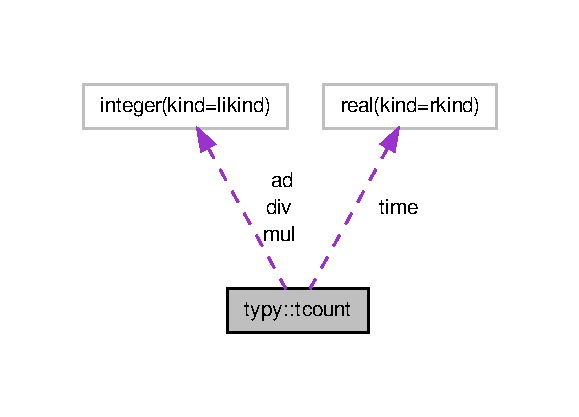
\includegraphics[width=278pt]{structtypy_1_1tcount__coll__graph}
\end{center}
\end{figure}
\subsection*{\-Public \-Attributes}
\begin{DoxyCompactItemize}
\item 
integer(kind=\hyperlink{classtypy_a2d07d3bd8360ffc201ade93859a7cc84}{likind}) \hyperlink{structtypy_1_1tcount_a76331414c9c7faa2ffcef099a188c5a0}{ad} = 0
\begin{DoxyCompactList}\small\item\em pocet aditivnich operaci \end{DoxyCompactList}\item 
integer(kind=\hyperlink{classtypy_a2d07d3bd8360ffc201ade93859a7cc84}{likind}) \hyperlink{structtypy_1_1tcount_acb3e84ceaddd7603add14a6a634be6ed}{mul} = 0
\begin{DoxyCompactList}\small\item\em pocet nasobeni \end{DoxyCompactList}\item 
integer(kind=\hyperlink{classtypy_a2d07d3bd8360ffc201ade93859a7cc84}{likind}) \hyperlink{structtypy_1_1tcount_a56f7ee9e379fb0657fc6729ae0e8eedc}{div} = 0
\begin{DoxyCompactList}\small\item\em pocet deleni \end{DoxyCompactList}\item 
real(kind=\hyperlink{classtypy_a2169287dfed38b596625c595cf3b5677}{rkind}) \hyperlink{structtypy_1_1tcount_a39ec51004274c0e7e2cd7142aa55cfcd}{time} = 0
\begin{DoxyCompactList}\small\item\em doba behu \end{DoxyCompactList}\end{DoxyCompactItemize}


\subsection{\-Detailed \-Description}
pocitadlo operaci 

\-Definition at line 15 of file typy.\-f90.



\subsection{\-Member \-Data \-Documentation}
\hypertarget{structtypy_1_1tcount_a76331414c9c7faa2ffcef099a188c5a0}{\index{typy\-::tcount@{typy\-::tcount}!ad@{ad}}
\index{ad@{ad}!typy::tcount@{typy\-::tcount}}
\subsubsection[{ad}]{\setlength{\rightskip}{0pt plus 5cm}integer(kind={\bf likind}) {\bf typy\-::tcount\-::ad} = 0}}\label{structtypy_1_1tcount_a76331414c9c7faa2ffcef099a188c5a0}


pocet aditivnich operaci 



\-Definition at line 17 of file typy.\-f90.

\hypertarget{structtypy_1_1tcount_a56f7ee9e379fb0657fc6729ae0e8eedc}{\index{typy\-::tcount@{typy\-::tcount}!div@{div}}
\index{div@{div}!typy::tcount@{typy\-::tcount}}
\subsubsection[{div}]{\setlength{\rightskip}{0pt plus 5cm}integer(kind={\bf likind}) {\bf typy\-::tcount\-::div} = 0}}\label{structtypy_1_1tcount_a56f7ee9e379fb0657fc6729ae0e8eedc}


pocet deleni 



\-Definition at line 21 of file typy.\-f90.

\hypertarget{structtypy_1_1tcount_acb3e84ceaddd7603add14a6a634be6ed}{\index{typy\-::tcount@{typy\-::tcount}!mul@{mul}}
\index{mul@{mul}!typy::tcount@{typy\-::tcount}}
\subsubsection[{mul}]{\setlength{\rightskip}{0pt plus 5cm}integer(kind={\bf likind}) {\bf typy\-::tcount\-::mul} = 0}}\label{structtypy_1_1tcount_acb3e84ceaddd7603add14a6a634be6ed}


pocet nasobeni 



\-Definition at line 19 of file typy.\-f90.

\hypertarget{structtypy_1_1tcount_a39ec51004274c0e7e2cd7142aa55cfcd}{\index{typy\-::tcount@{typy\-::tcount}!time@{time}}
\index{time@{time}!typy::tcount@{typy\-::tcount}}
\subsubsection[{time}]{\setlength{\rightskip}{0pt plus 5cm}real(kind={\bf rkind}) {\bf typy\-::tcount\-::time} = 0}}\label{structtypy_1_1tcount_a39ec51004274c0e7e2cd7142aa55cfcd}


doba behu 



\-Definition at line 23 of file typy.\-f90.



\-The documentation for this type was generated from the following file\-:\begin{DoxyCompactItemize}
\item 
\hyperlink{typy_8f90}{typy.\-f90}\end{DoxyCompactItemize}

\hypertarget{classtypy}{\section{typy \-Module \-Reference}
\label{classtypy}\index{typy@{typy}}
}


zakladni typy  




\-Collaboration diagram for typy\-:\nopagebreak
\begin{figure}[H]
\begin{center}
\leavevmode
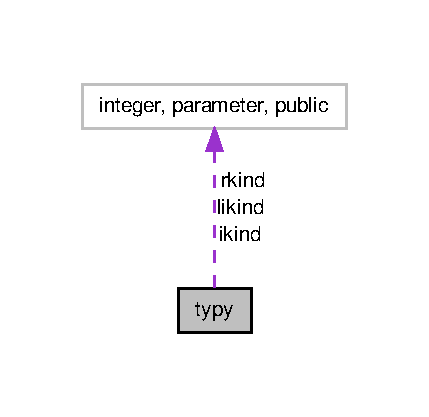
\includegraphics[width=206pt]{classtypy__coll__graph}
\end{center}
\end{figure}
\subsection*{\-Data \-Types}
\begin{DoxyCompactItemize}
\item 
type \hyperlink{structtypy_1_1tcount}{tcount}
\begin{DoxyCompactList}\small\item\em pocitadlo operaci \end{DoxyCompactList}\end{DoxyCompactItemize}
\subsection*{\-Public \-Member \-Functions}
\begin{DoxyCompactItemize}
\item 
subroutine, public \hyperlink{classtypy_a33123a40a2f37a906b69811afdae4451}{print\-\_\-info} (info)
\begin{DoxyCompactList}\small\item\em vytiskne udaje o pocitani \end{DoxyCompactList}\end{DoxyCompactItemize}
\subsection*{\-Public \-Attributes}
\begin{DoxyCompactItemize}
\item 
integer, parameter, public \hyperlink{classtypy_a2169287dfed38b596625c595cf3b5677}{rkind} = selected\-\_\-real\-\_\-kind(18, 99)
\begin{DoxyCompactList}\small\item\em kind pro realna cisla 18 cifer \end{DoxyCompactList}\item 
integer, parameter, public \hyperlink{classtypy_a80b310812529ce60b2aec26670db402c}{ikind} = selected\-\_\-int\-\_\-kind(10)
\begin{DoxyCompactList}\small\item\em kind pro cela cisla 10 cifer \end{DoxyCompactList}\item 
integer, parameter, public \hyperlink{classtypy_a2d07d3bd8360ffc201ade93859a7cc84}{likind} = selected\-\_\-int\-\_\-kind(16)
\begin{DoxyCompactList}\small\item\em velmi dlouha cela cisla \end{DoxyCompactList}\end{DoxyCompactItemize}


\subsection{\-Detailed \-Description}
zakladni typy 

\-Definition at line 6 of file typy.\-f90.



\subsection{\-Member \-Function/\-Subroutine \-Documentation}
\hypertarget{classtypy_a33123a40a2f37a906b69811afdae4451}{\index{typy@{typy}!print\-\_\-info@{print\-\_\-info}}
\index{print\-\_\-info@{print\-\_\-info}!typy@{typy}}
\subsubsection[{print\-\_\-info}]{\setlength{\rightskip}{0pt plus 5cm}subroutine, public {\bf typy\-::print\-\_\-info} (
\begin{DoxyParamCaption}
\item[{type({\bf tcount}), intent(in)}]{info}
\end{DoxyParamCaption}
)}}\label{classtypy_a33123a40a2f37a906b69811afdae4451}


vytiskne udaje o pocitani 



\-Definition at line 29 of file typy.\-f90.



\subsection{\-Member \-Data \-Documentation}
\hypertarget{classtypy_a80b310812529ce60b2aec26670db402c}{\index{typy@{typy}!ikind@{ikind}}
\index{ikind@{ikind}!typy@{typy}}
\subsubsection[{ikind}]{\setlength{\rightskip}{0pt plus 5cm}integer, parameter, public {\bf typy\-::ikind} = selected\-\_\-int\-\_\-kind(10)}}\label{classtypy_a80b310812529ce60b2aec26670db402c}


kind pro cela cisla 10 cifer 



\-Definition at line 10 of file typy.\-f90.

\hypertarget{classtypy_a2d07d3bd8360ffc201ade93859a7cc84}{\index{typy@{typy}!likind@{likind}}
\index{likind@{likind}!typy@{typy}}
\subsubsection[{likind}]{\setlength{\rightskip}{0pt plus 5cm}integer, parameter, public {\bf typy\-::likind} = selected\-\_\-int\-\_\-kind(16)}}\label{classtypy_a2d07d3bd8360ffc201ade93859a7cc84}


velmi dlouha cela cisla 



\-Definition at line 12 of file typy.\-f90.

\hypertarget{classtypy_a2169287dfed38b596625c595cf3b5677}{\index{typy@{typy}!rkind@{rkind}}
\index{rkind@{rkind}!typy@{typy}}
\subsubsection[{rkind}]{\setlength{\rightskip}{0pt plus 5cm}integer, parameter, public {\bf typy\-::rkind} = selected\-\_\-real\-\_\-kind(18, 99)}}\label{classtypy_a2169287dfed38b596625c595cf3b5677}


kind pro realna cisla 18 cifer 



\-Definition at line 8 of file typy.\-f90.



\-The documentation for this module was generated from the following file\-:\begin{DoxyCompactItemize}
\item 
\hyperlink{typy_8f90}{typy.\-f90}\end{DoxyCompactItemize}

\chapter{\-File \-Documentation}
\hypertarget{datasetup_8f90}{\section{datasetup.\-f90 \-File \-Reference}
\label{datasetup_8f90}\index{datasetup.\-f90@{datasetup.\-f90}}
}


konstruktory matic  


\subsection*{\-Data \-Types}
\begin{DoxyCompactItemize}
\item 
module \hyperlink{classdatasetup}{datasetup}
\begin{DoxyCompactList}\small\item\em konstruktory matic \end{DoxyCompactList}\end{DoxyCompactItemize}


\subsection{\-Detailed \-Description}
konstruktory matic 

\-Definition in file \hyperlink{datasetup_8f90_source}{datasetup.\-f90}.


\hypertarget{main_8f90}{\section{main.\-f90 \-File \-Reference}
\label{main_8f90}\index{main.\-f90@{main.\-f90}}
}


hlavni program  


\subsection*{\-Functions/\-Subroutines}
\begin{DoxyCompactItemize}
\item 
program \hyperlink{main_8f90_a86135f03075c1d51f0ffa1f750f6f86e}{pokus}
\begin{DoxyCompactList}\small\item\em hlavni program \end{DoxyCompactList}\end{DoxyCompactItemize}


\subsection{\-Detailed \-Description}
hlavni program 

\-Definition in file \hyperlink{main_8f90_source}{main.\-f90}.



\subsection{\-Function/\-Subroutine \-Documentation}
\hypertarget{main_8f90_a86135f03075c1d51f0ffa1f750f6f86e}{\index{main.\-f90@{main.\-f90}!pokus@{pokus}}
\index{pokus@{pokus}!main.f90@{main.\-f90}}
\subsubsection[{pokus}]{\setlength{\rightskip}{0pt plus 5cm}program {\bf pokus} (
\begin{DoxyParamCaption}
{}
\end{DoxyParamCaption}
)}}\label{main_8f90_a86135f03075c1d51f0ffa1f750f6f86e}


hlavni program 



\-Definition at line 6 of file main.\-f90.


\hypertarget{mtx_8f90}{\section{mtx.\-f90 \-File \-Reference}
\label{mtx_8f90}\index{mtx.\-f90@{mtx.\-f90}}
}


\-Objektova implementace matic.  


\subsection*{\-Data \-Types}
\begin{DoxyCompactItemize}
\item 
module \hyperlink{classmtx}{mtx}
\begin{DoxyCompactList}\small\item\em module pro matice \end{DoxyCompactList}\item 
type \hyperlink{structmtx_1_1matrix}{mtx\-::matrix}
\begin{DoxyCompactList}\small\item\em obecna matice \end{DoxyCompactList}\item 
interface \hyperlink{interfacemtx_1_1geti}{mtx\-::geti}
\begin{DoxyCompactList}\small\item\em interface pro ziskani prvku \end{DoxyCompactList}\item 
interface \hyperlink{interfacemtx_1_1seti}{mtx\-::seti}
\begin{DoxyCompactList}\small\item\em interface pro nastaveni prvku \end{DoxyCompactList}\item 
interface \hyperlink{interfacemtx_1_1ini}{mtx\-::ini}
\begin{DoxyCompactList}\small\item\em interface pro inicializaci=vymazani matice a resize \end{DoxyCompactList}\item 
type \hyperlink{structmtx_1_1fullmtx}{mtx\-::fullmtx}
\begin{DoxyCompactList}\small\item\em plna matice \end{DoxyCompactList}\item 
type \hyperlink{structmtx_1_1elemt}{mtx\-::elemt}
\begin{DoxyCompactList}\small\item\em typ pro prvek ridke matice \end{DoxyCompactList}\item 
type \hyperlink{structmtx_1_1smtx}{mtx\-::smtx}
\begin{DoxyCompactList}\small\item\em ridka matice \end{DoxyCompactList}\end{DoxyCompactItemize}


\subsection{\-Detailed \-Description}
\-Objektova implementace matic. 

\-Definition in file \hyperlink{mtx_8f90_source}{mtx.\-f90}.


\hypertarget{solvers_8f90}{\section{solvers.\-f90 \-File \-Reference}
\label{solvers_8f90}\index{solvers.\-f90@{solvers.\-f90}}
}


ruzne resice soustav linearnich rovnic  


\subsection*{\-Data \-Types}
\begin{DoxyCompactItemize}
\item 
module \hyperlink{classsolvers}{solvers}
\begin{DoxyCompactList}\small\item\em resice soustav \end{DoxyCompactList}\end{DoxyCompactItemize}


\subsection{\-Detailed \-Description}
ruzne resice soustav linearnich rovnic 

\-Definition in file \hyperlink{solvers_8f90_source}{solvers.\-f90}.


\hypertarget{typy_8f90}{\section{typy.\-f90 \-File \-Reference}
\label{typy_8f90}\index{typy.\-f90@{typy.\-f90}}
}


modul pro zakladni typy  


\subsection*{\-Data \-Types}
\begin{DoxyCompactItemize}
\item 
module \hyperlink{classtypy}{typy}
\begin{DoxyCompactList}\small\item\em zakladni typy \end{DoxyCompactList}\item 
type \hyperlink{structtypy_1_1tcount}{typy\-::tcount}
\begin{DoxyCompactList}\small\item\em pocitadlo operaci \end{DoxyCompactList}\end{DoxyCompactItemize}


\subsection{\-Detailed \-Description}
modul pro zakladni typy 

\-Definition in file \hyperlink{typy_8f90_source}{typy.\-f90}.


\printindex
\end{document}
